\chapter{Definições Preliminares}

Neste capítulo, reunimos as noções matemáticas básicas necessárias para compreensão completa do texto.

Fixaremos notações e conceitos (conjuntos, relações, funções, digrafos, propriedade em digrafos, digrafos ponderados, ramificações geradoras, arborescências, funções de custo, dualidade, problemas duais e algoritmos), até chegar à formulação do problema da r-arborescência inversa de custo mínimo e adiamos descrições algorítmicas para capítulos posteriores.

\section{Conjuntos}

Este trabalho depende profundamente da teoria dos conjuntos, podemos dizer que todos os objetos matemáticos que iremos utilizar nessa dissertação se reduzem a conjuntos e operações entre eles.


Um \textbf{conjunto} é uma agregação de objetos distintos com características bem definidas, chamados elementos ou membros do conjunto. Os conjuntos são geralmente representados por letras maiúsculas (por exemplo, \(A\), \(B\), \(C\)) e seus elementos são listados entre chaves (por exemplo, \(A = \{1, 2, 3\}\)). Dois conjuntos são iguais se contêm exatamente os mesmos elementos.


Podemos ter conjuntos de qualquer tipo de objeto, incluindo números, letras e elementos da natureza. Para motivar as definições ao longo do texto, usaremos dois exemplos complementares que vamos chamar de exemplos-mestres:
\begin{itemize}
	\item (i) Considere um universo \(U\) composto por três conjuntos: árvores \(T\), plantas \(P\) e fungos \(F\) — para praticar pertinência, inclusão e operações; e

	      \begin{figure}[H]
		      \centering
		      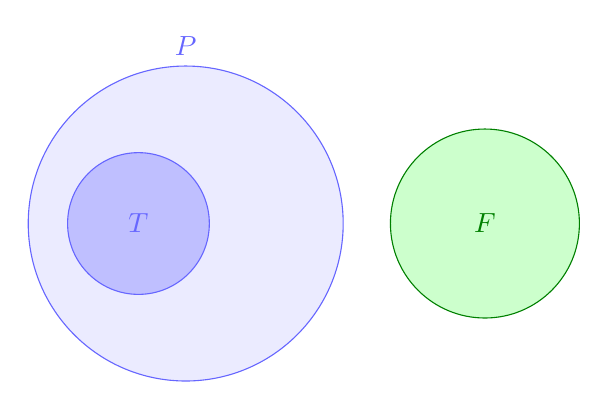
\begin{tikzpicture}[scale=1]
			      % Conjuntos P, T e F
			      % P: plantas (círculo maior)
			      \draw[fill=blue!8, draw=blue!60] (0,0) circle (2);
			      \node[blue!60] at (0,2.25) {$P$};
			      % T: árvores (círculo menor dentro de P)
			      \draw[fill=blue!25, draw=blue!60] (-0.6,0) circle (0.9);
			      \node[blue!60] at (-0.6,0) {$T$};
			      % F: fungos (círculo disjunto)
			      \draw[fill=green!20, draw=green!50!black] (3.8,0) circle (1.2);
			      \node[green!50!black] at (3.8,0) {$F$};
		      \end{tikzpicture}
		      \caption{Relações entre os conjuntos de organismos: $T\subseteq P$ (toda árvore é planta) e $F$ é disjunto de $P$.}
		      \label{fig:organismos}
	      \end{figure}

	\item (ii) exemplo inspirado na navalha de Occam, com três famílias: evidências \(E\), hipóteses \(H\) e explicações \(\mathcal{M} \subseteq 2^{H}\). Nesse segundo exemplo, privilegiaremos explicações parcimoniosas: entre as que cobrem \(E\), preferimos as minimais por inclusão.
\end{itemize}


No segundo exemplo, consideremos \(E=\{\text{queda de temperatura},\, \text{céu nublado}\}\) e \(H=\{H_A, H_B\}\), em que \(H_A\) significa “frente fria” e \(H_B\), “ilha de calor”. Tanto \(\{H_A\}\) quanto \(\{H_A,H_B\}\) explicam \(E\) (cobrem ambas as evidências), mas, por parcimônia, preferimos \(\{H_A\}\), por ser estritamente menor do que \(\{H_A,H_B\}\) (\(\{H_A\} \subset \{H_A,H_B\}\)). Ao longo do texto, recorreremos às noções de pertinência (por exemplo, \(H_A\in H\)), de inclusão e às operações usuais sobre conjuntos (união, interseção etc.) para comparar explicações.

\begin{figure}[htbp]
	\centering
	\begin{tikzpicture}[>=Stealth, node distance=1.6cm]
		% Evidências
		\node[draw, rounded corners, fill=gray!10, minimum width=3.8cm] (E1) {queda de temperatura};
		\node[draw, rounded corners, fill=gray!10, minimum width=3.8cm, below=of E1] (E2) {céu nublado};
		% Hipóteses
		\node[draw, rounded corners, fill=orange!20, left=4.2cm of E1, minimum width=3.2cm] (HA) {$H_A$: frente fria};
		\node[draw, rounded corners, fill=orange!10, below=of HA, minimum width=3.2cm] (HB) {$H_B$: ilha de calor};
		% Setas de cobertura
		\draw[->, thick] (HA.east) -- (E1.west);
		\draw[->, thick] (HA.east) -- (E2.west);
		\draw[->, dashed] (HB.east) -- (E2.west);
		% Nota de parcimônia
		\node[align=center, font=\small, below=1.0cm of E2] (nota) {Ambas as opções $H_A$ e $H_A + H_B$ cobrem $E$;\\ por parcimônia, preferimos apenas $H_A$.};
	\end{tikzpicture}
	\caption{\texorpdfstring{Exemplo inspirado na navalha de Occam: $H_A$ cobre ambas as evidências ($E$), enquanto $H_B$ seria redundante; prefere-se a explicação menor.}{Exemplo inspirado na navalha de Occam}}
	\label{fig:occam-exemplo}
\end{figure}


\subsection{Subconjuntos}

Dizemos que \(A\) é um \textbf{subconjunto} de \(B\), denotado \(A \subseteq B\), quando todo elemento de \(A\) também pertence a \(B\). Se, além disso, \(A \neq B\), escrevemos \(A \subset B\) e chamamos \(A\) de \textbf{subconjunto próprio} de \(B\). Ex.: \( \{1,2\} \subseteq \{1,2,3\} \) e \( \{1,2\} \subset \{1,2,3\} \).Por convenção, o conjunto vazio \(\varnothing\) é subconjunto de qualquer conjunto \(X\) (isto é, \(\varnothing \subseteq X\)), e todo conjunto é subconjunto de si mesmo (\(X \subseteq X\)).


No primeiro exemplo-mestre, sejam \(P\) o conjunto de plantas, \(T\) o de árvores e \(F\) o de fungos; então \(T \subseteq P\) (toda árvore é planta), ao passo que \(F \not\subseteq P\).


No segundo, seja \(H=\{H_A, H_B\}\) e \(E=\{\text{queda de temperatura},\, \text{céu nublado}\}\), vale \(\{H_A\} \subset \{H_A,H_B\} \subseteq H\); ambas as opções explicam \(E\), mas,
por parcimônia, preferimos \(\{H_A\}\).

\subsection{Pertinência e inclusão}


Pertinência e inclusão são os conceitos mais fundamentais da teoria dos conjuntos.


Começando pela \textbf{noção de pertinência} denotado por \(\in\): dizemos que um elemento \(x\) pertence a um conjunto \(X\) quando \(x \in X\) e não pertence quando \(x \notin X\).


Seja o nosso universo \(U\) de organismos: \(P=\{\text{todas as plantas}\}\), \(T=\{\text{todas as árvores}\}\) e \(F=\{\text{todos os fungos}\}\). Se \(x\) é um carvalho, então \(x\in T\) e, como toda árvore é uma planta, \(x\in P\). Já se \(y\) é um cogumelo, então \(y\in F\) e, na taxonomia moderna, \(y\notin T\) e \(y\notin P\). Agora, considere \(A=\{\text{árvores com folhas verdes}\}\); a pertinência fica clara: \(x\in A\) se, e somente se, \(x\) é árvore e tem folhas verdes.


\begin{figure}[H]
	\centering
	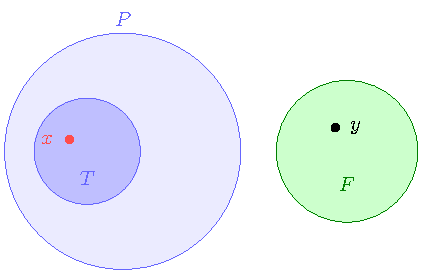
\includegraphics[width=0.9\linewidth]{figures/fig_pertinencia.pdf}

	\caption{Pertinência: $x\in T\subseteq P$ (ponto vermelho dentro de $T$) e $y\in F$ (ponto preto); logo $y\notin P$ e $y\notin T$.}
	\label{fig:pertinencia}\end{figure}



Continuando, vem a \textbf{relação de inclusão} entre conjuntos denotada por \(\subseteq\): escrevemos \(X \subseteq Y\) quando todo elemento de \(X\) também pertence a \(Y\) (e \(X\subset Y\) quando, além disso, \(X\neq Y\)). No nosso exemplo, \(A\subseteq T\subset P\) e \(T\cap F=\varnothing\) (árvores e fungos não se sobrepõem).


\begin{figure}[H]
	\centering
	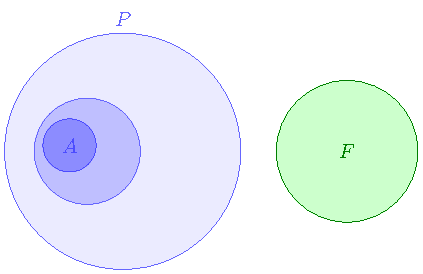
\includegraphics[width=0.9\linewidth]{figures/fig_inclusao.pdf}

	\caption{\texorpdfstring{Inclusão: $A\subseteq T\subset P$ (círculos aninhados) e $T\cap F=\varnothing$ (círculos disjuntos).}{Inclusão: conjuntos aninhados e disjuntos}}
	\label{fig:inclusao}\end{figure}


\subsection{Operações entre conjuntos}

Com essas definições de pertinência, inclusão e subconjuntos, apresentamos as operações básicas entre conjuntos, que usaremos ao longo do texto (mantendo o exemplo com \(P,T,F,A\)).

Outras operações comuns entre conjuntos incluem:
\begin{itemize}
	\item \textbf{União} (\(A \cup B\)): o conjunto de todos os elementos que pertencem a \(A\), a \(B\), ou ambos.

	      Exemplo: \(T \cup F\) é o conjunto de todos os organismos que são árvores ou fungos (ou ambos, se existissem tais organismos).
	      \begin{figure}[H]
		      \centering
		      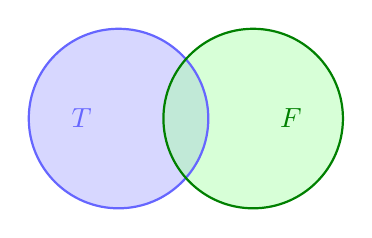
\begin{tikzpicture}[scale=0.95]
			      % União T ∪ F com sobreposição visível (interseção)
			      \def\r{1.2}
			      \coordinate (LT) at (-0.9,0);
			      \coordinate (LF) at (0.9,0);
			      % Preenchimento semitransparente para evidenciar a interseção
			      \fill[blue!35, opacity=0.45] (LT) circle (\r);
			      \fill[green!35, opacity=0.45] (LF) circle (\r);
			      % Contornos e rótulos
			      \draw[thick, blue!60] (LT) circle (\r) node[left=6pt] {$T$};
			      \draw[thick, green!50!black] (LF) circle (\r) node[right=6pt] {$F$};
		      \end{tikzpicture}
		      \caption{União: a área colorida representa $T \cup F$; a sobreposição evidencia a interseção $T \cap F$ (hipotética).}
		      \label{fig:op-uniao}
	      \end{figure}


	\item \textbf{União disjunta} (\(A \uplus B\)): o conjunto de todos os elementos que pertencem a \(A\) ou a \(B\), mas não a ambos; é igual a \(A \cup B\) quando \(A\) e \(B\) são disjuntos.

	      Exemplo: \(T \uplus F\) é o conjunto de todos os organismos que são árvores ou fungos, mas não ambos (o que é trivialmente igual a \(T \cup F\) pois \(T\) e \(F\) são disjuntos).
	      \begin{figure}[H]
		      \centering
		      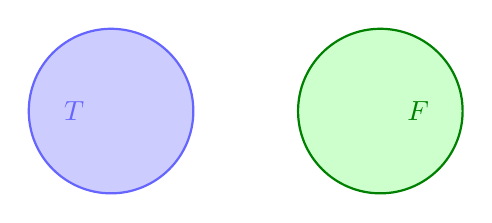
\begin{tikzpicture}[scale=0.95]
			      \def\r{1.1}
			      \coordinate (LT) at (-1.8,0);
			      \coordinate (LF) at (1.8,0);
			      \fill[blue!20] (LT) circle (\r);
			      \fill[green!20] (LF) circle (\r);
			      \draw[thick, blue!60] (LT) circle (\r) node[left=6pt] {$T$};
			      \draw[thick, green!50!black] (LF) circle (\r) node[right=6pt] {$F$};
		      \end{tikzpicture}
		      \caption{União disjunta: como $T \cap F= \varnothing$, tem-se $T \uplus F = T \cup F$.}
		      \label{fig:op-uniao-disjunta}
	      \end{figure}


	\item \textbf{Interseção} (\(A \cap B\)): o conjunto de todos os elementos que pertencem tanto a \(A\) quanto a \(B\).

	      Exemplo: \(T \cap P = T\), pois todas as árvores são plantas.
	      \begin{figure}[H]
		      \centering
		      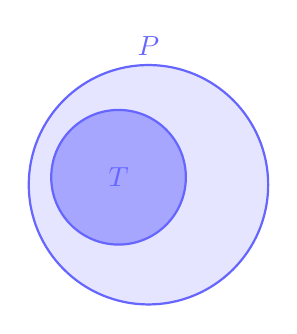
\begin{tikzpicture}[scale=0.95]
			      % Interseção T ∩ P = T (T ⊆ P)
			      \def\rP{1.6}
			      \def\rT{0.9}
			      \coordinate (cP) at (0,0);
			      \coordinate (cT) at (-0.4,0.1);
			      % P (maior) e T (dentro de P)
			      \draw[fill=blue!10, draw=blue!60, thick] (cP) circle (\rP);
			      \node[blue!60] at (0,\rP+0.25) {$P$};
			      % Preencher T (interseção equivale a T)
			      \draw[fill=blue!35, draw=blue!60, thick] (cT) circle (\rT);
			      \node[blue!60] at (cT) {$T$};
		      \end{tikzpicture}
		      \caption{Interseção: como $T \subseteq P$, $T \cap P = T$ (a região escura é $T$).}
		      \label{fig:op-intersecao}
	      \end{figure}


	\item \textbf{Diferença} (\(A \setminus B\)): o conjunto de todos os elementos que pertencem a \(A\) mas não a \(B\).

	      Exemplo: \(T \setminus A\) é o conjunto de todas as árvores que não têm folhas verdes.
	      \begin{figure}[H]
		      \centering
		      \begin{tikzpicture}[scale=0.95]
			      % Diferença T \ A (A ⊆ T)
			      \def\rT{1.4}
			      \def\rA{0.8}
			      \coordinate (cT) at (0,0);
			      \coordinate (cA) at (0.4,0.2);
			      % Preencher T
			      \draw[fill=blue!25, draw=blue!60, thick] (cT) circle (\rT);
			      % Remover a parte A de dentro de T
			      \begin{scope}
				      \clip (cT) circle (\rT);
				      \fill[white] (cA) circle (\rA);
			      \end{scope}
			      \draw[thick, blue!60] (cT) circle (\rT) node[above right=2pt and -2pt] {$T$};
			      \draw[thick, blue!60] (cA) circle (\rA) node[right=4pt] {$A$};
		      \end{tikzpicture}
		      \caption{Diferença: região azul representa $T \setminus A$ (árvores que não têm folhas verdes).}
		      \label{fig:op-diferenca}
	      \end{figure}


	\item \textbf{Complemento} de \(X\) em um universo fixo \(U\): \(X^c := U\setminus X\) (também chamado de \textit{complemento absoluto}); o \textit{complemento relativo} de \(X\) em \(Y\) é \(Y\setminus X\).

	      Exemplo: \(T^c = U \setminus T\) é o conjunto de todos os organismos que não são árvores. Ou seja, \(T^c\) inclui plantas que não são árvores, fungos e quaisquer outros organismos no universo \(U\).
	      \begin{figure}[H]
		      \centering
		      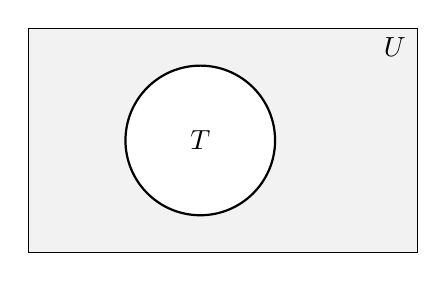
\begin{tikzpicture}[scale=0.95]
			      % Universo U e conjunto T
			      \draw[fill=gray!10, draw=black] (-2.6,-1.5) rectangle (2.6,1.5);
			      \draw[fill=white, draw=black, thick] (-0.3,0) circle (1.0);
			      \node at (-0.3,0) {$T$};
			      \node at (2.3,1.25) {$U$};
		      \end{tikzpicture}
		      \caption{Complemento: a área cinza representa $T^c = U \setminus T$.}
		      \label{fig:op-complemento}
	      \end{figure}


	\item \textbf{Diferença simétrica} (\(A\,\Delta\, B\)): \((A\setminus B)\cup(B\setminus A)\); é igual a \(A\cup B\) quando \(A\) e \(B\) são disjuntos.

	      Exemplo: \(P\,\Delta\, F\) é o conjunto de todos os organismos que são plantas ou fungos, mas não ambos (o que é trivialmente igual a \(P \cup F\) pois \(P\) e \(F\) são disjuntos).
	      \begin{figure}[H]
		      \centering
		      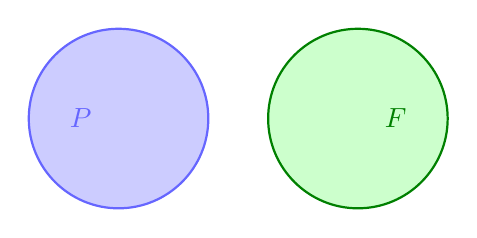
\begin{tikzpicture}[scale=0.95]
			      % Diferença simétrica P Δ F com P e F disjuntos
			      \def\r{1.2}
			      \coordinate (LP) at (-1.6,0);
			      \coordinate (LF) at (1.6,0);
			      \fill[blue!20] (LP) circle (\r);
			      \fill[green!20] (LF) circle (\r);
			      \draw[thick, blue!60] (LP) circle (\r) node[left=6pt] {$P$};
			      \draw[thick, green!50!black] (LF) circle (\r) node[right=6pt] {$F$};
		      \end{tikzpicture}
		      \caption{Diferença simétrica: como $P \cap F= \varnothing$, temos $P\, \Delta\, F = P \cup F$.}
		      \label{fig:op-dif-simetrica}
	      \end{figure}


	\item \textbf{Produto cartesiano} (\(A\times B\)): o conjunto de pares ordenados \((a,b)\) com \(a\in A\) e \(b\in B\).

	      Exemplo: \(T=\{t_1,t_2\}\) e \(F=\{f_1,f_2\}\). Então \(T\times F = \{(t_1,f_1),(t_1,f_2),(t_2,f_1),(t_2,f_2)\}\).
	      \begin{figure}[H]
		      \centering
		      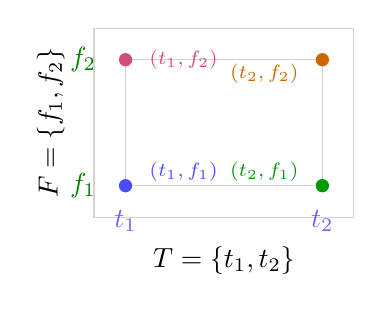
\begin{tikzpicture}[scale=1]
			      % Grade limpa para T × F (2×2) sem sobreposições
			      \def\xone{0}
			      \def\xtwo{2.5}
			      \def\yone{0}
			      \def\ytwo{1.6}
			      % Moldura e linhas da grade
			      \draw[gray!35] (\xone-0.4,\yone-0.4) rectangle (\xtwo+0.4,\ytwo+0.4);
			      \draw[gray!35] (\xone,\yone) -- (\xone,\ytwo);
			      \draw[gray!35] (\xtwo,\yone) -- (\xtwo,\ytwo);
			      \draw[gray!35] (\xone,\yone) -- (\xtwo,\yone);
			      \draw[gray!35] (\xone,\ytwo) -- (\xtwo,\ytwo);
			      % Pontos de T×F com cores distintas por par
			      \fill[blue!70] (\xone,\yone) circle (2.4pt);   % (t1,f1)
			      \fill[purple!70] (\xone,\ytwo) circle (2.4pt); % (t1,f2)
			      \fill[green!60!black] (\xtwo,\yone) circle (2.4pt); % (t2,f1)
			      \fill[orange!80!black] (\xtwo,\ytwo) circle (2.4pt); % (t2,f2)
			      % Rótulos dos pares (posicionados para não sobrepor)
			      \node[font=\scriptsize, text=blue!70, anchor=west]  at (\xone+0.18,\yone+0.18) {$(t_1,f_1)$};
			      \node[font=\scriptsize, text=purple!70, anchor=west] at (\xone+0.18,\ytwo) {$(t_1,f_2)$};
			      \node[font=\scriptsize, text=green!60!black, anchor=east] at (\xtwo-0.18,\yone+0.18) {$(t_2,f_1)$};
			      \node[font=\scriptsize, text=orange!80!black, anchor=east] at (\xtwo-0.18,\ytwo-0.18) {$(t_2,f_2)$};
			      % Rótulos dos elementos
			      \node[blue!60] at (\xone,\yone-0.45) {$t_1$};
			      \node[blue!60] at (\xtwo,\yone-0.45) {$t_2$};
			      \node[green!50!black, anchor=east] at (\xone-0.25,\yone) {$f_1$};
			      \node[green!50!black, anchor=east] at (\xone-0.25,\ytwo) {$f_2$};
			      % Rótulos dos conjuntos (eixos)
			      \node at (0.5*\xtwo, -0.95) {$T=\{t_1,t_2\}$};
			      \node[rotate=90] at (\xone-0.95, 0.5*\ytwo) {$F=\{f_1,f_2\}$};
		      \end{tikzpicture}
		      \caption{Produto cartesiano: pontos representam os pares de $T \times F$ para $T=\{t_1,t_2\}$ e $F=\{f_1,f_2\}$.}
		      \label{fig:op-produto}
	      \end{figure}


	\item \textbf{Conjunto das partes} (\(2^U\)): a família de todos os subconjuntos de \(U\) (inclui \(\varnothing\) e o próprio \(U\)).

	      Exemplo: se \(U = \{x,y\}\), então \(2^U = \{\varnothing, \{x\}, \{y\}, \{x,y\}\}\). Logo, \(|2^U|=4=2^{|U|}\).
	      \begin{figure}[H]
		      \centering
		      \begin{tikzpicture}[scale=1, node distance=0.9cm]
			      % Diagrama de Hasse para U={x,y}
			      \node (empty) at (0,0) {$\varnothing$};
			      \node (x) [above left=of empty] {$\{x\}$};
			      \node (y) [above right=of empty] {$\{y\}$};
			      \node (xy) [above=of empty] {$\{x,y\}$};
			      \draw (empty) -- (x) -- (xy) -- (y) -- (empty);
		      \end{tikzpicture}
		      \caption{Conjunto das partes: diagrama de Hasse de $2^{U}$ para $U=\{x,y\}$.}
		      \label{fig:op-partes}
	      \end{figure}
\end{itemize}

\subsubsection{Identidades úteis.}
Usaremos livremente as propriedades clássicas de conjuntos — comutatividade e associatividade de \(\cup\) e \(\cap\), distributividade e as \textbf{leis de De Morgan} — sem prova. Quando for relevante, explicitaremos a identidade no ponto de uso. Por exemplo, no nosso universo \(U\), \((P\cup F)^c = P^c\cap F^c\).

\subsection{Coleção}


Entre os objetos que podem pertencer a um conjunto, estão também eles mesmos, outros conjuntos. Chamaremos tais conjuntos de \textbf{coleções} (ou \textbf{famílias}) de conjuntos. Por exemplo, \(\mathcal{C} = \{P, T, F\}\) é uma coleção formada pelos conjuntos de organismos já definidos: plantas \(P\), árvores \(T\) e fungos \(F\). Note que \(\mathcal{C}\) é um conjunto como outro qualquer; seus elementos são, cada um, um conjunto.


Coleções são úteis para agrupar subconjuntos relacionados de um mesmo universo. Por exemplo, considere \(\mathcal{D} = \{A, B\}\), onde \(A = \{\text{árvores com folhas verdes}\}\) e \(B = \{\text{árvores com folhas vermelhas}\}\). Assim, \(\mathcal{D} \subseteq 2^{T}\) é uma coleção de subconjuntos de \(T\).


Uma coleção \(\mathcal{F}\) é dita \textbf{laminar} quando, para quaisquer \(X, Y \in \mathcal{F}\), vale que \(X \subseteq Y\), \(Y \subseteq X\) ou \(X \cap Y = \varnothing\); isto é, quaisquer dois conjuntos são aninhados (um está contido no outro) ou são disjuntos.


Por exemplo, na coleção \(\mathcal{C} = \{P, T, F\}\): \(P\) é o conjunto de todas as plantas, \(T\) o de todas as árvores (portanto \(T\subseteq P\)) e \(F\) o de todos os fungos (disjunto de plantas e, logo, de árvores). Assim, quaisquer dois conjuntos em \(\mathcal{C}\) são aninhados ou disjuntos, e \(\mathcal{C}\) é laminar. Na coleção \(\mathcal{D} = \{A, T\}\): \(A\) é o conjunto de árvores com folhas verdes e \(T\) o de todas as árvores; como toda árvore de \(A\) é árvore de \(T\), temos \(A\subseteq T\) e a coleção é laminar. Já em \(\mathcal{E} = \{A, R\}\): \(R\) é o conjunto de árvores frutíferas; há árvores que são ao mesmo tempo frutíferas e de folhas verdes (a interseção é não vazia), mas nenhuma das classes contém a outra, então \(\mathcal{E}\) não é laminar.


\begin{figure}[H]
	\centering
	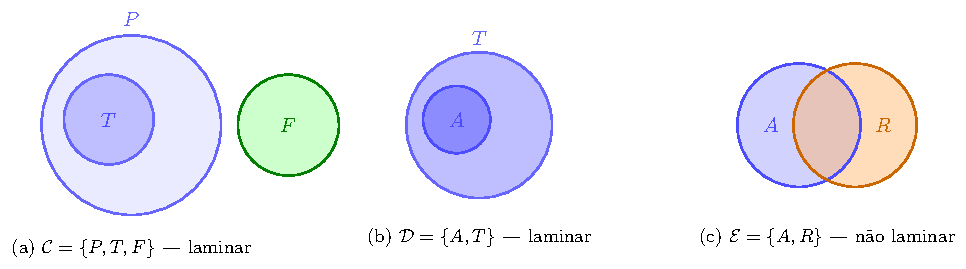
\includegraphics[width=0.9\linewidth]{figures/fig_laminaridade.pdf}

	\caption{Laminaridade em coleções: em (a) e (b), quaisquer dois conjuntos são aninhados ou disjuntos; em (c), $A$ e $R$ se interceptam sem inclusão, violando a laminaridade.}
	\label{fig:laminaridade}\end{figure}



Este é um importante conceito que aparecerá no restante do trabalho. A ideia de laminaridade retornará quando tratarmos de cortes dirigidos.

\subsection{Comparando conjuntos: cardinalidade e maximalidade}


Podemos comparar conjuntos através de relações de tamanho (cardinalidade) ou por relações de inclusão. Essas duas formas de comparação são distintas e importantes, especialmente quando lidamos com coleções de conjuntos.


A \textbf{cardinalidade} de um conjunto \(A\), denotada por \(|A|\), é o número de elementos de \(A\). Para conjuntos finitos, é simplesmente a contagem dos elementos (por exemplo, se \(A=\{1,2,3\}\), então \(|A|=3\)). Para conjuntos infinitos, a cardinalidade pode ser mais complexa, envolvendo conceitos como infinito enumerável e não enumerável. Por exemplo, o conjunto dos números naturais \(\mathbb{N}\) é infinito enumerável, enquanto o conjunto dos números reais \(\mathbb{R}\) é infinito não enumerável.


Dizemos que \(A\in\mathcal{C}\) tem \textbf{maior cardinalidade} se \(|A|\ge |B|\) para todo \(B\in\mathcal{C}\) (podendo haver empates). Esse critério não coincide, em geral, com a comparação por relação de inclusão. Em grafos, por exemplo, distinguem-se conjuntos independentes \emph{maximais} (não ampliáveis) de conjuntos independentes \emph{máximos} (de cardinalidade máxima).


Ao compararmos uma coleção \(\mathcal{C}\) de conjuntos utilizando sua relações de inclusão \((\mathcal{C},\subseteq)\), é imprescindível distinguir \textbf{maximal} de \textbf{máximo}.


Um conjunto \(A\in\mathcal{C}\) é \textbf{maximal} se não existe \(B\in\mathcal{C}\) tal que \(A\subset B\). Em palavras: não dá para ampliar \(A\) estritamente dentro da coleção. Podem haver vários elementos maximais, e eles podem ser incomparáveis entre si. Ex.: em \(\mathcal{C}=\big\{\{1\},\{2\}\big\}\), ambos \(\{1\}\) e \(\{2\}\) são maximais, mas não existe máximo.


Um conjunto \(A\in\mathcal{C}\) é \textbf{máximo} se \(B\subseteq A\) para todo \(B\in\mathcal{C}\). Se existe, é único. Ex.: em \(\mathcal{C}=\big\{\{1\},\{2\},\{1,2\}\big\}\), o conjunto \(\{1,2\}\) é o máximo.


Um bom exemplo para ilustrar a distinção entre conjuntos maximais e máximos é a coleção \(\mathcal{C}=\big\{\{1\},\{2\},\{1,2\},\{3\}\big\}\). Aqui, \(\{1,2\}\) é o único conjunto máximo (contém todos os outros), enquanto \(\{1\}\), \(\{2\}\) e \(\{3\}\) são todos maximais (não podem ser ampliados dentro da coleção).


Esses conceitos reaparecerão ao longo do texto, especialmente na diferença entre estruturas \textbf{maximais} (saturadas por inclusão) e \textbf{máximas/ótimas} (de maior cardinalidade ou menor custo). Para fixar ideias:
\begin{itemize}
	\item Em muitos problemas, “\textbf{maximal}” quer dizer: não dá para ampliar uma escolha sem violar as regras; já “\textbf{máximo/ótimo}” quer dizer: entre todas as escolhas válidas, essa é a melhor segundo o critério (por exemplo, menor custo).
	\item No algoritmo de \textbf{Chu--Liu/Edmonds}, começamos com escolhas locais que já não podem ser ampliadas dentro das regras do problema e, a partir delas, chegamos a uma solução de menor custo.
	\item No método de \textbf{András Frank}, primeiro construímos uma estrutura organizada que garante escolhas suficientes; depois, usando apenas relações já ativadas por essa estrutura, extraímos a solução ótima.
	\item Moral: partimos da ideia de “não dá para aumentar” (maximal) e chegamos a “melhor possível” (máximo/ótimo). Os detalhes técnicos de cada método aparecerão nas seções próprias.
\end{itemize}

\section{Relações e Funções}


Desde a introdução, vimos a ideia filosófica de explicar como “ligar” fatos a hipóteses da forma mais parcimoniosa possível. Para tornar essa intuição precisa, precisamos de uma linguagem que descreva objetos (conjuntos) e como eles se conectam. É aqui que entram as \textbf{relações} e, de modo ainda mais disciplinado, as \textbf{funções}: regras que associam a cada elemento de um conjunto exatamente um elemento de outro. Com elas, passamos do discurso qualitativo sobre explicações para uma estrutura matemática que permite medir, comparar e, adiante, otimizar.


Para tornar essa discussão prática, desenvolvemos uma aplicação \textit{web} interativa que permite visualizar passo a passo o funcionamento dos dois algoritmos, destacando suas diferenças e semelhanças. A seguir, discutimos a dimensão didática que motivou essas escolhas e como fundamentos de aprendizagem e visualização embasam o projeto.


Uma \textbf{relação} \(R\) entre dois conjuntos \(A\) e \(B\) é um subconjunto do produto cartesiano \(A \times B\). Ou seja, \(R \subseteq A \times B\). Se \((a,b) \in R\), dizemos que \(a\) está relacionado a \(b\) pela relação \(R\), denotado \(aRb\).


\begin{figure}[H]
	\centering
	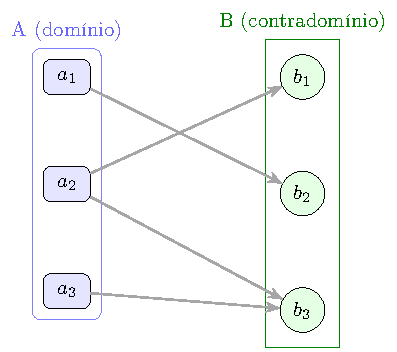
\includegraphics[width=0.9\linewidth]{figures/fig_relacao.pdf}

	\caption{Relação $R\subseteq A\times B$. Cada seta representa um par $(a,b)\in R$ (isto é, $a\,R\,b$). As formas/cores distinguem domínio ($A$, retângulos azuis) de contradomínio ($B$, círculos verdes). Note que $a_2$ se relaciona com $b_1$ e $b_3$; logo, este $R$ \emph{não é função}.}
	\label{fig:relacao}
\end{figure}



No nosso primeiro exemplo-mestre, considere \(P=\{\text{todas as plantas}\}\) e \(F=\{\text{todos os fungos}\}\). Definimos a relação \(R\) como ``é um organismo que compete com''. Assim, se uma planta \(p \in P\) compete com um fungo \(f \in F\), então \((p,f) \in R\).


No nosso segundo exemplo, considere \(H=\{\text{hipóteses}\}\) e \(E=\{\text{evidências}\}\). Definimos a relação \(R\) como ``explica''. Se uma hipótese \(h \in H\) explica uma evidência \(e \in E\), então \((h,e) \in R\).


Em teoria dos grafos, uma relação pode representar conexões entre vértices. Por exemplo, em um grafo dirigido, a relação ``existe uma aresta de \(u\) para \(v\)'' pode ser representada como um conjunto de pares ordenados \((u,v)\).


Uma \textbf{função} \(f\) de um conjunto \(A\) em um conjunto \(B\) é uma relação especial que associa cada elemento de \(A\) a exatamente um elemento de \(B\). Denotamos isso como \(f: A \to B\). Se \(f(a) = b\), dizemos que \(b\) é a imagem de \(a\) sob \(f\).


\begin{figure}[H]
	\centering
	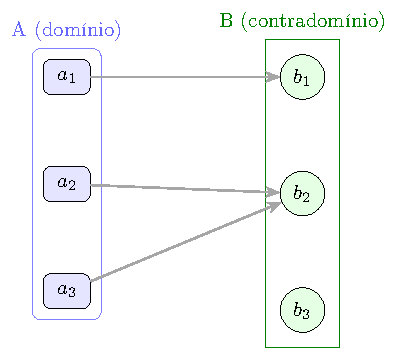
\includegraphics[width=0.9\linewidth]{figures/fig_funcao.pdf}

	\caption{Função $f\!:\!A\to B$. Cada elemento de $A$ tem \emph{exatamente uma} imagem em $B$.}
	\label{fig:funcao}
\end{figure}



No nosso exemplo-mestre, considere \(P=\{\text{todas as plantas}\}\) e \(\mathbb{N}=\{0,1,2,\ldots\}\) (números naturais). Definimos a função \(f: P \to \mathbb{N}\) que associa cada planta ao seu número de folhas. Se \(p \in P\) é uma árvore com 100 folhas, então \(f(p) = 100\).


Em teoria dos grafos, funções podem ser usadas para atribuir valores numéricos --- também chamados de pesos ou custos --- às arestas. Por exemplo, se temos um grafo \(G\) com arestas \(e_1, e_2, \ldots, e_n\), podemos definir uma função \(c: E \to \mathbb{R}^+\) que atribui um peso \(c(e_i)\) a cada aresta \(e_i\).


Na ciência da computação, relações e funções são usadas para modelar conexões entre dados, estruturas de dados e operações. Por exemplo, em bancos de dados relacionais, tabelas representam relações entre diferentes entidades. Em programação funcional, funções são tratadas como cidadãos de primeira classe, permitindo a criação de funções de ordem superior que podem receber outras funções como argumentos ou retorná-las como resultados.

\subsection{Conceitos em Funções}

Alguns conceitos importantes relacionados a funções incluem:
\begin{itemize}
	\item \textbf{Domínio}: o conjunto \(A\) de entrada da função \(f: A \to B\).
	\item \textbf{Contradomínio}: o conjunto \(B\) de possíveis saídas da função.
	\item \textbf{Imagem}: o conjunto de valores efetivamente atingidos pela função, \(f(A) = \{f(a) \mid a \in A\}\).

	      \begin{figure}[H]
		      \centering
		      \begin{tikzpicture}[>=Stealth, node distance=1.1cm]
			      % Elementos do domínio A (retângulos azuis)
			      \node[draw, rounded corners, fill=blue!10, minimum width=9mm, minimum height=6mm] (a1img) {$a_1$};
			      \node[draw, rounded corners, fill=blue!10, below=of a1img, minimum width=9mm, minimum height=6mm] (a2img) {$a_2$};
			      \node[draw, rounded corners, fill=blue!10, below=of a2img, minimum width=9mm, minimum height=6mm] (a3img) {$a_3$};
			      % Elementos do contradomínio B (círculos verdes)
			      \node[circle, draw, fill=green!10, right=3.2cm of a1img, minimum size=6mm] (b1img) {$b_1$};
			      \node[circle, draw, fill=green!10, below=of b1img, minimum size=10mm] (b2img) {$b_2$};
			      \node[circle, draw, fill=green!10, below=of b2img, minimum size=6mm] (b3img) {$b_3$};
			      % Caixas de agrupamento com rótulos
			      \node[draw=blue!50, rounded corners, fit=(a1img)(a2img)(a3img), inner sep=5pt, label={[blue!60]above:A (domínio)}] {};
			      \node[draw=green!50!black, fit=(b1img)(b2img)(b3img), inner sep=7pt, label={[green!50!black]above:B (contradomínio)}] {};
			      % Setas de f (exatamente uma por elemento de A)
			      \draw[->, thick, draw=gray!70] (a1img) -- (b1img);
			      \draw[->, thick, draw=gray!70] (a2img) -- (b2img);
			      \draw[->, thick, draw=gray!70] (a3img) -- (b2img);
			      % Destaque da imagem f(A) ⊆ B
			      \node[draw=purple!70!black, thick, fit=(b1img)(b2img), inner sep=3pt, label distance=15mm, label={[purple!70!black]right:Imagem $f(A)$}] {};
		      \end{tikzpicture}
		      \caption{Domínio, contradomínio e imagem: $A$ (retângulos azuis) mapeia via $f$ para $B$ (círculos verdes). A imagem $f(A)$ é o subconjunto de $B$ efetivamente atingido (aqui, $\{b_1,b_2\}$).}
		      \label{fig:dom-contradom-imagem}
	      \end{figure}

	\item \textbf{Injetora}: uma função \(f\) é injetora se \(f(a_1) = f(a_2)\) implica \(a_1 = a_2\); ou seja, elementos distintos do domínio têm imagens distintas.
	\item \textbf{Sobrejetora}: uma função \(f\) é sobrejetora se para todo \(b \in B\), existe \(a \in A\) tal que \(f(a) = b\); ou seja, a imagem é igual ao contradomínio.
	\item \textbf{Bijetora}: uma função que é tanto injetora quanto sobrejetora; estabelece uma correspondência um-para-um entre os elementos de \(A\) e \(B\).

\end{itemize}


\begin{figure}[H]
	\centering
	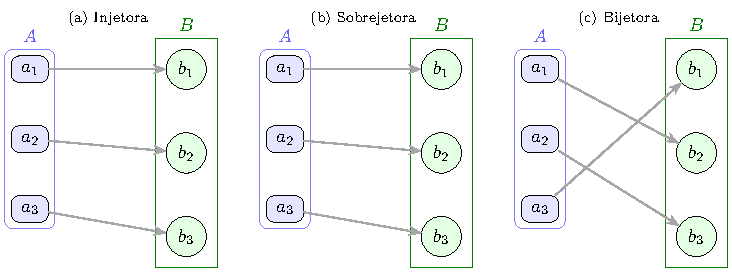
\includegraphics[width=0.9\linewidth]{figures/fig_inj_sobre_bij.pdf}

	\caption{Funções especiais: (a) Injetora — elementos distintos em $A$ têm imagens distintas em $B$; (b) Sobrejetora — todo elemento de $B$ é imagem; (c) Bijetora — um-para-um e sobre $B$.}
	\label{fig:inj-sobre-bij}\end{figure}


\subsection{Funções de agregação e somatórios}


Além de relacionar elementos de conjuntos, muitas operações familiares em matemática, envolvem \emph{funções} que recebem coleções de números (ou funções) e devolvem um número.


Uma \textbf{função de agregação} é uma função que recebe um conjunto (ou sequência) de valores e retorna um único valor que representa algum aspecto agregado desses valores. Exemplos comuns incluem:
\begin{itemize}
	\item \textbf{Média}: A média aritmética de um conjunto de números \(x_1, x_2, \ldots, x_n\) é dada por \(\frac{1}{n}\sum_{i=1}^{n} x_i\).
	\item \textbf{Máximo e Mínimo}: A função máximo retorna o maior valor em um conjunto, enquanto a função mínimo retorna o menor valor.
	\item \textbf{Produto}: O produto de um conjunto de números \(x_1, x_2, \ldots, x_n\) é dado por \(\prod_{i=1}^{n} x_i\).
	\item \textbf{Contagem}: A função contagem retorna o número de elementos em um conjunto.
\end{itemize}

O \textbf{somatório}, por exemplo, é uma função de agregação linear que mapeia uma sequência \((x_1,\dots,x_n)\) em sua soma:
\[\sum_{i=1}^{n} x_i.\]

Esse conceito é especialmente útil em otimização e em análise combinatória: somatórios aparecem o tempo todo e serão explorados ao longo deste trabalho.

\subsubsection{Exemplos com grafos.}
As sessões seguintes explorarão em maiores detalhes grafos e digrafos, mas agora, consideremos a ideia básica: um \textbf{grafo} é um conjunto de pontos (\emph{vértices}) ligados por linhas (\emph{arestas}). No caso \emph{não dirigido}, as linhas não têm seta; no caso \emph{dirigido}, cada linha tem um sentido e é chamada de \emph{arco}.


A noção de somatória aparecerá naturalmente quando lidamos com propriedades dos grafos. Por exemplo:

Seja um grafo não dirigido \(G=(V,E)\). O \textbf{grau} de um vértice \(v\in V\), escrito \(\deg(v)\), é quantas arestas tocam em \(v\). A soma dos graus de todos os vértices conta cada aresta \emph{duas vezes} (uma por extremidade), portanto:
\[\sum_{v\in V} \deg(v) = 2\,|E|.\]

Em grafos dirigidos, distinguimos \(\deg^{-}(v)\) (quantos arcos \emph{chegam} em \(v\)) e \(\deg^{+}(v)\) (quantos arcos \emph{saem} de \(v\)). Cada arco contribui com 1 para um grau de saída e 1 para um grau de entrada, logo:
\[\sum_{v\in V} \deg^{-}(v) = \sum_{v\in V} \deg^{+}(v) = |E|.\]


Agora suponha que cada aresta/arco \(e\in E\) tenha um \emph{peso} (ou \emph{custo}) \(c(e)\ge 0\). O \textbf{custo total} de um subconjunto \(F\subseteq E\) é simplesmente a soma dos pesos das arestas escolhidas:
\[C(F) = \sum_{e\in F} c(e).\]
De maneira análoga, se \(X\subseteq V\) é um conjunto de vértices, o \textbf{valor total} (ou peso total) dos arcos que \emph{saem} de \(X\) é a soma dos pesos dessas setas. Usaremos mais adiante a notação \(\delta^{+}(X)\) para o conjunto de arcos que saem de \(X\) (ver a seção de digrafos); com essa notação,
\[\operatorname{val}^+(X) = \sum_{e\in \delta^{+}(X)} c(e).\]
Esses exemplos mostram como somatórios capturam propriedades estruturais do grafo por meio de funções simples de agregação.

\subsection{Funções Especiais}

\subsubsection{Função de custo}
Uma \textbf{função de custo} é uma função \(c: A \to \mathbb{R}^+\) que atribui um valor numérico não negativo (custo) a cada elemento de um conjunto \(A\). Essas funções são amplamente utilizadas em otimização, economia e teoria dos grafos para modelar despesas, penalidades ou recursos associados a escolhas ou ações.


Exemplo: Considere um conjunto de tarefas \(T = \{t_1, t_2, t_3\}\). Uma função de custo \(c: T \to \mathbb{R}^+\) pode ser definida como:
\[c(t_1) = 5, \quad c(t_2) = 10, \quad c(t_3) = 3.\]
Aqui, \(c(t_i)\) representa o custo de realizar a tarefa \(t_i\).


Depende diretamente do conceito de somatório, pois frequentemente queremos minimizar o custo total de um conjunto de escolhas. Se \(S \subseteq A\) é um subconjunto de elementos escolhidos, o custo total associado a \(S\) é dado por:
\[C(S) = \sum_{a \in S} c(a).\]

\subsubsection{Função c-disjunta}
Uma \textbf{função c-disjunta} é uma função \(f: A \to B\) que, para quaisquer \(a_1, a_2 \in A\) com \(a_1 \neq a_2\), as imagens \(f(a_1)\) e \(f(a_2)\) são disjuntas, ou seja, \(f(a_1) \cap f(a_2) = \varnothing\). Em outras palavras, elementos distintos do domínio são mapeados para conjuntos disjuntos no contradomínio.


\begin{figure}[H]
	\centering
	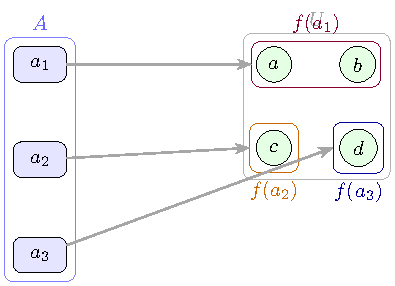
\includegraphics[width=0.9\linewidth]{figures/fig_c_disjunta.pdf}

	\caption{Função c-disjunta: cada \(a\in A\) mapeia para um \emph{subconjunto} de $B$, e imagens de elementos distintos são disjuntas.}
	\label{fig:c-disjunta}
\end{figure}



Exemplo: Considere \(A = \{1, 2, 3\}\) e \(B = \{\{a\}, \{b\}, \{c\}, \{d\}\}\). Definimos a função \(f: A \to B\) como:
\[f(1) = \{a, b\}, \quad f(2) = \{c\}, \quad f(3) = \{d\}.\]
Aqui, \(f\) é c-disjunta, pois \(f(1) \cap f(2) = \varnothing\), \(f(1) \cap f(3) = \varnothing\) e \(f(2) \cap f(3) = \varnothing\).

\subsubsection{Função c-viável}

Uma \textbf{função c-viável} é uma função \(g: A \to \mathbb{R}^+\) que satisfaz certas condições de viabilidade relacionadas a um conjunto de restrições ou critérios. Essas funções são frequentemente usadas em otimização e teoria dos grafos para garantir que as soluções propostas atendam a requisitos específicos.

Exemplo: Considere um conjunto de projetos \(P = \{p_1, p_2, p_3\}\) e uma função \(g: P \to \mathbb{R}^+\) que atribui um valor de viabilidade a cada projeto. Suponha que temos a restrição de que a soma dos valores de viabilidade deve ser menor ou igual a um certo limite \(L\). Se definirmos:
\[g(p_1) = 4, \quad g(p_2) = 6, \quad g(p_3) = 3,\]
então a função \(g\) é c-viável se \(g(p_1) + g(p_2) + g(p_3) \leq L\).
Essas funções são essenciais para garantir que as soluções propostas em problemas de otimização sejam práticas e atendam aos critérios estabelecidos.

\subsubsection{Funções de otimização}


Do ponto de vista semiótico, “melhor” exprime uma preferência entre interpretações: ao comparar alternativas, escolhemos aquela cuja significação é mais adequada a um critério. Para tornar isso operacional, a matemática troca “fazer mais sentido” por “ter maior (ou menor) valor” em uma escala formal: fixamos (i) um conjunto de soluções viáveis \(\mathcal{F}\) e (ii) uma função numérica sobre \(\mathcal{F}\) que induz uma ordem de comparação.


Formalmente, usamos uma \textbf{função objetivo} (ou \textbf{função de otimização})
\[h:\; \mathcal{F} \to \mathbb{R},\]
que atribui um número real a cada solução. Buscamos uma solução \(S^*\in\mathcal{F}\) que \emph{minimize} ou \emph{maximize} \(h\) (isto é, um \(\operatorname*{argmin}\) ou \(\operatorname*{argmax}\)). Quando esse número resulta da soma de contribuições elementares, obtemos o caso aditivo, em ligação direta com os somatórios apresentados antes.


Caso \emph{aditivo}. Quando cada elemento \(a\in A\) tem um custo \(c(a)\ge 0\) e as soluções são subconjuntos \(S\subseteq A\), a função objetivo mais comum é o custo total
\[C(S)=\sum_{a\in S} c(a),\]
que desejamos \emph{minimizar}. De modo análogo, se cada item tem um benefício \(p(a)\ge 0\), podemos \emph{maximizar} o benefício total \(P(S)=\sum_{a\in S} p(a)\), possivelmente sujeito a restrições (por exemplo, de orçamento ou limite).


Outro exemplo: considere produtos \(X=\{x_1,x_2,x_3\}\) com lucro \(p(x_1)=10\), \(p(x_2)=15\), \(p(x_3)=7\). Se houver um limite de custo que impede escolher todos, o objetivo típico é escolher um subconjunto \(S\subseteq X\) que maximize \(\sum_{x\in S} p(x)\) respeitando as restrições. Essa forma reflete exatamente os somatórios introduzidos antes.


Em todos os casos, a função objetivo explicita o critério de “melhor”, e as restrições determinam quais soluções são aceitáveis.

\subsection{Otimização}

O princípio da navalha de occam nos diz que a explicação mais simples tende a ser a correta. Do ponto de vista semiótico, isso é escolher, entre interpretações possíveis, a que melhor satisfaz um critério. A matemática também se preocupa com identificar a “melhor” solução entre várias alternativas, mas traduz essa ideia em termos quantitativos: fixamos (i) um conjunto de soluções viáveis \(\mathcal{F}\) e (ii) uma função numérica sobre \(\mathcal{F}\) que induz uma ordem de comparação.


Assim, a otimização envolve a maximização ou minimização de uma função objetivo \(h: \mathcal{F} \to \mathbb{R}\) sobre um conjunto de soluções viáveis \(\mathcal{F}\).


Esse conceito pode aparecer em muitas necessidades do dia-a-dia: uma empresa pode querer minimizar custos de produção, um viajante pode buscar o caminho mais curto entre dois pontos, ou um investidor pode tentar maximizar o retorno de um portfólio. Em cada caso, a função objetivo quantifica o que significa ser “melhor” ou “mais eficiente”.


Pensando em modelagem de problemas em grafos, podemos pensar em exemplos clássicos de otimização:

\begin{itemize}
	\item \textbf{Caminho mais curto}: Dado um grafo com pesos nas arestas, encontrar o caminho entre dois vértices que minimize a soma dos pesos das arestas percorridas.
	\item \textbf{Árvore geradora mínima}: Encontrar uma árvore que conecte todos os vértices de um grafo com o menor custo total das arestas.
	\item \textbf{Fluxo máximo}: Em um grafo direcionado com limites nas arestas, encontrar o fluxo máximo que pode ser enviado de uma fonte a um sumidouro sem exceder esses limites.
\end{itemize}

\subsection{A dualidade}


O taoísmo chinês fala do yin e yang, forças opostas que se complementam. Um conceito que remete à contrastes, noite e dia, matéria e anti-matéria, máximos e mínimos. Na matemática, um conceito semelhante é a \emph{dualidade}, que conecta problemas de minimização a problemas de maximização.


Em termos matemáticos, para cada problema de otimização (o \emph{primal}), existe um problema associado (o \emph{dual}) que oferece uma perspectiva complementar. Resolver um desses problemas pode fornecer insights ou soluções para o outro.

\subsubsection{Exemplo:}
Considere um problema de otimização onde queremos minimizar o custo de transporte de mercadorias entre diferentes armazéns. O problema primal busca a solução de transporte que minimize os custos totais, enquanto o problema dual pode ser formulado como a maximização do valor dos recursos disponíveis (como a capacidade dos armazéns e a demanda dos clientes).


No nosso texto, consideramos como problema primal a minimização do custo de uma estrutura (como uma árvore geradora mínima) e como dual a maximização de um conjunto de pesos ou preços que justificam esse custo mínimo. A relação entre primal e dual é formalizada por teoremas de dualidade, que garantem que o valor ótimo do primal é igual ao valor ótimo do dual sob certas condições.


Esse ponto de vista leva a “teoremas min–max” que ligam problemas de \emph{minimização} a problemas de \emph{maximização} e fornecem certificados verificáveis de otimalidade.


\begin{figure}[H]
	\centering
	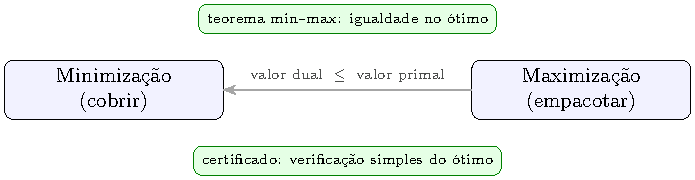
\includegraphics[width=0.9\linewidth]{figures/fig_min_max_cert.pdf}

	\caption{Intuição de min--max: um problema de cobrir (minimização) e um de empacotar (maximização) andam juntos. Sempre vale valor dual $\le$ valor primal; quando há igualdade, temos um certificado de otimalidade.}
	\label{fig:min-max-cert}\end{figure}


Uma forma didática de ver a dualidade (no caso linear) é a seguinte. Temos um conjunto de soluções possíveis (um poliedro)
\[P=\{x\in\mathbb{R}^n:\ Ax\ge b\},\]
e um vetor \(c\in\mathbb{R}^n\) que mede o \emph{custo} de cada coordenada de \(x\); o valor da solução é a soma ponderada \(c^\top x\). O problema \textbf{dual} escolhe \(y\ge 0\) (um “preço” para cada restrição de \(Ax\ge b\)) exigindo que nenhuma variável fique “subprecificada”: isso é expresso por
\[A^\top y\ \le\ c.\]
Com essa única condição, todo \(y\ge 0\) fornece automaticamente um \textbf{limitante inferior} para \(c^\top x\) em todo \(P\):
\[c^\top x\ \ge\ (A^\top y)^\top x\ =\ y^\top(Ax)\ \ge\ y^\top b.\]
Geometricamente, \(y^\top b\) é o nível de um \emph{hiperplano de suporte} que nunca ultrapassa a função objetivo \(c^\top x\) sobre \(P\).

No \textbf{ótimo}, existem \(x\) (primal) e \(y\) (dual) viáveis com o \emph{mesmo} valor
\[c^\top x\ =\ y^\top b,\]
isto é, o “vão de dualidade” é zero. Além disso, valem as condições de \textbf{complementaridade}, que dizem “onde há folga de um lado, há zero do outro”:
\[x\odot\big(c-A^\top y\big)=0\quad\text{e}\quad y\odot\big(Ax-b\big)=0.
\]
Interpretando:
\begin{itemize}
	\item Se \(x_j>0\), então o \emph{custo reduzido} daquela coordenada é nulo: \(c_j-(A^\top y)_j=0\). Caso contrário, pode haver folga \(c_j>(A^\top y)_j\) e a variável fica em zero.
	\item Se \(y_i>0\), então a \(i\)-ésima restrição está “apertada” (sem folga): \((Ax-b)_i=0\). Caso contrário, se há folga \((Ax-b)_i>0\), o preço \(y_i\) zera.
\end{itemize}
Essas igualdades capturam a intuição central: o dual estabelece preços que justificam o valor mínimo do primal, e as soluções ótimas usam apenas “direções” cujo custo reduzido é zero e apoiam-se em restrições ativas.


No contexto de grafos, a otimização costuma aparecer como a busca por subestruturas (caminhos, árvores, cortes, fluxos) que minimizam ou maximizam um custo, sempre respeitando a topologia do grafo.


Nesta dissertação, essa noção de otimização é central: olhamos para o mesmo problema por dois ângulos que se completam. No lado “primal”, queremos montar diretamente a arborescência de menor custo. O algoritmo de Chu–Liu/Edmonds faz isso de forma gulosa: ajusta os custos por vértice, cria arestas de custo zero (0-arestas), contrai ciclos quando aparecem e segue até montar a solução ótima.
(\cite{chu1965,edmonds1967optimum}).


No lado “dual”, em vez de montar a árvore, colocamos custos em cortes do grafo com raiz $r$. A regra é simples: nenhum custo pode ultrapassar o custo das arestas que cruzam o corte. Buscamos escolher esses custos para somar o máximo possível. As arestas que “batem no limite” viram 0-arestas, e a partir delas conseguimos reconstruir uma arborescência ótima. Essa visão, desenvolvida por Frank, leva a um teorema min–max e a um procedimento em duas etapas: primeiro ajustamos os custos, depois extraímos a solução usando apenas 0-arestas.
(cf. \cite{frank2014,schrijver2003comb})

\section{Problemas interessantes}


Qual o número mínimo de cores necessárias para colorir um mapa de países, de modo que países vizinhos tenham cores diferentes? Qual o caminho mais curto entre duas cidades em um mapa rodoviário? Como encontrar a árvore geradora mínima que conecta todas as cidades com o menor custo total? Essas perguntas são exemplos clássicos de problemas que podem ser modelados e resolvidos usando a teoria dos grafos. Vistas sob a lente da navalha de occam, todas elas buscam a solução mais parcimoniosa que atende ao requisito: usar poucas cores, percorrer um caminho curto ou conectar tudo com custo mínimo.


\begin{figure}[H]
	\centering
	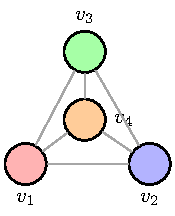
\includegraphics[width=0.9\linewidth]{figures/fig_coloracao.pdf}

	\caption{Coloração de grafos: exemplo de coloração própria do grafo completo $K_4$. Como $K_4$ é completo, precisamos de 4 cores para colorir seus vértices de modo que vértices adjacentes tenham cores diferentes. Uma coloração é uma função $\varphi:V\to C$ tal que, se $uv\in E$, então $\varphi(u)\neq\varphi(v)$.}
	\label{fig:coloracao}\end{figure}



Sem a teoria dos grafos, seria difícil formalizar e resolver esses problemas de maneira eficiente. Ao representar situações do mundo real como grafos, tornamos a parcimônia da navalha de occam algo operacional: escolhemos uma medida simples (número de cores, comprimento, custo) e aplicamos algoritmos que, entre as soluções viáveis, minimizam ou maximizam esse critério — produzindo soluções ótimas ou, quando necessário, boas aproximações.

\section{Grafos}

Falamos bastante de grafos ao longo do texto, aqui fixamos a noção básica.


Um \textbf{grafo} \(G = (V, E)\) é uma estrutura matemática composta por um conjunto \(V\) de \emph{vértices} (ou \emph{nós}) e um conjunto \(E\) de \emph{arestas} (ou \emph{ligações}) que conectam pares de vértices.


\begin{figure}[H]
	\centering
	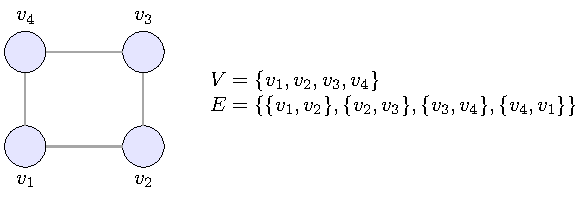
\includegraphics[width=0.9\linewidth]{figures/fig_def_grafo.pdf}

	\caption{Definição de grafo: exemplo de grafo simples \(G=(V,E)\). Pontos representam os vértices \(V\) e linhas representam as arestas \(E\), que são pares não ordenados de vértices distintos.}
	\label{fig:def-grafo}\end{figure}



O conjunto de vértices \(V\) pode ser definido como \(V = \{v_1, v_2, \ldots, v_n\}\), onde cada \(v_i\) representa um ponto distinto no grafo. O conjunto de arestas \(E\) é um conjunto de pares não ordenados de vértices, ou seja, \(E \subseteq \{\{u, v\} \mid u, v \in V, u \neq v\}\). Cada aresta \(\{u, v\}\) indica uma conexão entre os vértices \(u\) e \(v\).


Esses vértices e arestas podem representar uma variedade de entidades e relações no mundo real. Por exemplo, em um grafo que modela uma rede social, os vértices podem representar pessoas, e as arestas podem representar amizades entre elas. Em um grafo que representa uma rede de transporte, os vértices podem ser cidades, e as arestas podem ser estradas ou rotas de voo conectando essas cidades.


Tendo em mente esses problemas, podemos falar de custos associados às arestas. Por exemplo, em um grafo que representa uma rede de transporte, cada aresta pode ter um custo associado, como a distância entre duas cidades ou o tempo necessário para percorrer uma estrada. Em um grafo que modela uma rede de comunicação, as arestas podem ter custos relacionados à largura de banda ou à latência.


Esses custos representam uma função \(c: E \to \mathbb{R}^+\) que atribui um valor numérico não negativo a cada aresta do grafo. Assim, para cada aresta \(\{u, v\} \in E\), \(c(\{u, v\})\) representa o custo associado a essa conexão.


\begin{figure}[H]
	\centering
	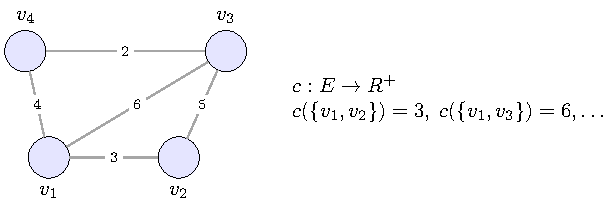
\includegraphics[width=0.9\linewidth]{figures/fig_grafo_custos.pdf}

	\caption{Grafo com custos nas arestas: a função $c:E\to\mathbb{R}^+$ atribui um custo não negativo a cada aresta.}
	\label{fig:grafo-custos}
\end{figure}



Grafos apresentam diversas estruturas especiais. Essas estruturas são definidas como subgrafos e são fundamentais para entender a topologia e as propriedades dos grafos, e muitas vezes são o foco de problemas de otimização.

\subsection{Subgrafos}
Um \textbf{subgrafo} \(H = (V_H, E_H)\) de um grafo \(G = (V, E)\) é um grafo cujos vértices e arestas são subconjuntos dos vértices e arestas de \(G\). Formalmente, \(V_H \subseteq V\) e \(E_H \subseteq E\), e cada aresta em \(E_H\) conecta dois vértices em \(V_H\).


Alguns subgrafos interessantes incluem: caminhos, ciclos, componentes conexas e árvores. Muitas propriedades e algoritmos em grafos dependem dessas estruturas, como encontrar o caminho mais curto entre dois vértices, detectar ciclos ou construir árvores geradoras mínimas. Dentre essas muitas estruturas especiais, vamos apresentar as que são relevantes para o desenvolvimento desta dissertação:

\subsubsection{Caminhos}
Um \textbf{caminho} em um grafo é uma sequência de vértices conectados por arestas. Formalmente, um caminho \(P\) de comprimento \(k\geq 1\) é uma sequência de vértices \(P = (v_1, v_2, \ldots, v_{k+1})\) tal que cada par consecutivo \((v_i, v_{i+1})\) é uma aresta em \(E\). O comprimento do caminho é o número de arestas que ele contém, que é \(k\).


\begin{figure}[H]
	\centering
	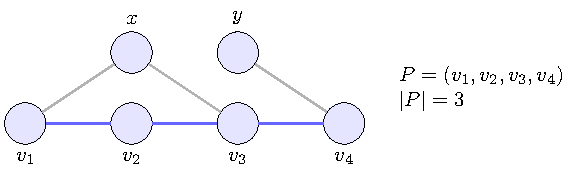
\includegraphics[width=0.9\linewidth]{figures/fig_caminho.pdf}

	\caption{Caminho em grafo não dirigido: o caminho $P=(v_1,v_2,v_3,v_4)$ está destacado em azul. Seu comprimento é o número de arestas percorridas, $|P|=3$.}
	\label{fig:caminho}\end{figure}


\subsubsection{Ciclos}
Um \textbf{ciclo} é um caminho que começa e termina no mesmo vértice, ou seja, \(v_1 = v_{k+1}\). Formalmente, um ciclo \(C\) é uma sequência de vértices \(C = (v_1, v_2, \ldots, v_k, v_1)\) tal que cada par consecutivo \((v_i, v_{i+1})\) é uma aresta em \(E\) e \(k \geq 2\). O comprimento do ciclo é o número de arestas que ele contém, que é \(k\).


\begin{figure}[H]
	\centering
	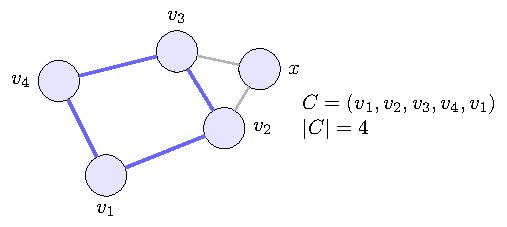
\includegraphics[width=0.9\linewidth]{figures/fig_ciclo.pdf}

	\caption{Ciclo em grafo não dirigido: o ciclo $C=(v_1,v_2,v_3,v_4,v_1)$ está destacado em azul. Seu comprimento é o número de arestas, $|C|=4$.}
	\label{fig:ciclo}\end{figure}


\subsubsection{Componentes conexas}
Uma \textbf{componente conexa} de um grafo é um subgrafo maximal que é conexo. Formalmente, uma componente conexa \(C\) é um subgrafo \(C = (V_C, E_C)\) onde \(V_C \subseteq V\) e \(E_C \subseteq E\), tal que \(C\) é conexo (existe um caminho entre qualquer par de vértices em \(V_C\)). Além disso, \(C\) é maximal, o que significa que não é possível adicionar mais vértices ou arestas a \(C\) sem perder a propriedade de conexidade.


\begin{figure}[H]
	\centering
	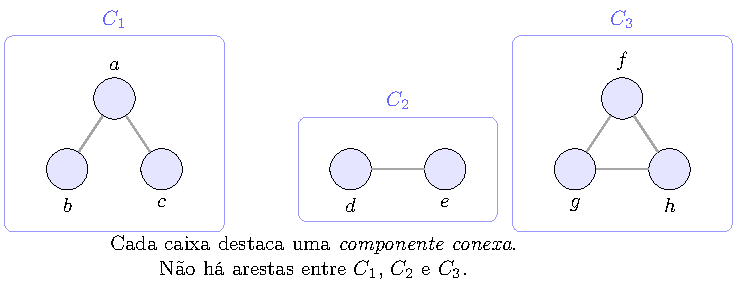
\includegraphics[width=0.9\linewidth]{figures/fig_componentes.pdf}

	\caption{Componentes conexas: o grafo possui três componentes $C_1$, $C_2$ e $C_3$. Cada $C_i$ é conexo e \emph{maximal}, isto é, não pode ser estendido mantendo a conexidade.}
	\label{fig:componentes}
\end{figure}


\subsubsection{Árvores}
Uma \textbf{árvore} é um grafo conexo e acíclico. Formalmente, uma árvore \(T\) é um grafo \(T = (V_T, E_T)\) onde \(V_T \subseteq V\) e \(E_T \subseteq E\), tal que \(T\) é conexo (existe um caminho entre qualquer par de vértices em \(V_T\)) e \(T\) é acíclico (não contém ciclos). Além disso, uma árvore com \(n\) vértices sempre tem exatamente \(n-1\) arestas.


\begin{figure}[H]
	\centering
	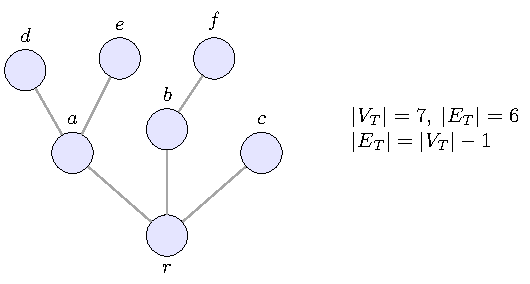
\includegraphics[width=0.9\linewidth]{figures/fig_arvore.pdf}

	\caption{Árvore: grafo conexo e acíclico. No exemplo, $|V_T|=7$ e $|E_T|=6$, satisfazendo $|E_T|=|V_T|-1$. Não há ciclos e existe um único caminho simples entre quaisquer dois vértices.}
	\label{fig:arvore}\end{figure}



Para o nosso objetivo principal, nos interessa entendê-las em grafos que a direção das conexões (arestas) importa.

\section{digrafos: quando a direção importa}

Existem problemas que a direção das arestas faz toda a diferença. Por exemplo, em uma rede de tráfego, algumas ruas são de mão única, ou em uma rede de comunicação, os dados podem ser enviados em uma direção específica. Nesses casos, usamos \emph{grafos dirigidos} (ou grafos direcionados ou simplesmente digrafos), onde as arestas são pares de vértices ordenados.


Um \textbf{grafo dirigido - digrafo} (grafos direcionados) é uma estrutura matemática composta por um conjunto \(V\) de \emph{vértices} e um conjunto \(A\) de \emph{arcos} (ou \emph{arestas direcionadas}) que conectam pares ordenados de vértices.


Por vértices entendemos o mesmo conjunto que em grafos comuns, mas agora as arestas entre eles têm uma direção específica. Cada arco \((u, v) \in A\) indica uma conexão direcionada do vértice \(u\) para o vértice \(v\), significando que a relação ou fluxo ocorre de \(u\) para \(v\).


Assim, temos os conceitos de cabeça e cauda de um arco: em \((u, v)\), \(u\) é a \emph{cauda} (origem) e \(v\) é a \emph{cabeça} (destino). Esses conceitos podem ser formalizados por meio de funções \(s, t: A \to V\), onde \(s((u, v)) = u\) (cauda) e \(t((u, v)) = v\) (cabeça).


\begin{figure}[H]
	\centering
	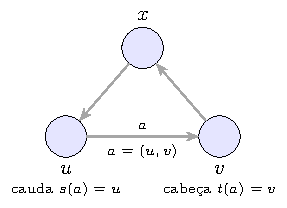
\includegraphics[width=0.9\linewidth]{figures/fig_def_digrafo.pdf}

	\caption{digrafos: arcos têm direção. No arco $a=(u,v)$, $u$ é a \emph{cauda} e $v$ é a \emph{cabeça}.}
	\label{fig:def-digrafo}
\end{figure}



Em digrafos podem ocorrer laços (arcos que conectam um vértice a ele mesmo, como \((u, u)\)) nesse caso as funções \(s\) e \(t\) coincidem. Também podem ocorrer múltiplos arcos entre o mesmo par de vértices (como \((u, v)\) e \((u, v)\) distintos). Pictograficamente representamos essas condições com setas com dupla ponta ou com rótulos diferentes.


\begin{figure}[H]
	\centering
	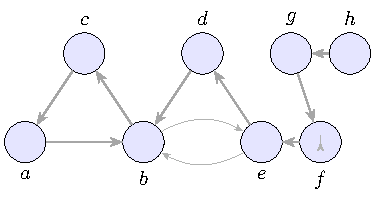
\includegraphics[width=0.9\linewidth]{figures/fig_def_digrafo_simples.pdf}

	\caption{digrafo: exemplo de grafo dirigido \(D=(V,A)\). Pontos representam os vértices \(V\) e setas representam os arcos \(A\), que são pares ordenados de vértices. Laços (como \((f,f)\)) e múltiplos arcos (como \((b,e)\) e \((e,b)\)) são permitidos.}
	\label{fig:def-digrafo-simples}\end{figure}



Tal qual os grafos comuns, os digrafos podem ter custos associados aos arcos. A função de custo \(c: A \to \mathbb{R}^+\) atribui um valor numérico geralmente não negativo a cada arco do digrafo. Assim, para cada arco \((u, v) \in A\), \(c((u, v))\) representa o custo associado a essa conexão direcionada.


\begin{figure}[H]
	\centering
	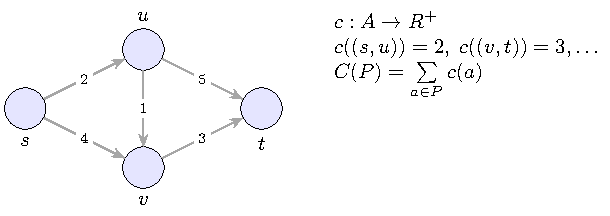
\includegraphics[width=0.9\linewidth]{figures/fig_digrafo_custos.pdf}

	\caption{digrafos com custos nos arcos: a função $c:A\to\mathbb{R}^+$ atribui um custo não negativo a cada arco.}
	\label{fig:digrafo-custos}
\end{figure}



Um conceito importante em digrafos é o de grau de um vértice. O \textbf{grau de entrada} (ou \emph{in-degree}) de um vértice \(v\), denotado por \(d^-(v)\), é o número de arcos que chegam a \(v\) (ou seja, o número de arcos cujo destino é \(v\)). O \textbf{grau de saída} (ou \emph{out-degree}) de um vértice \(v\), denotado por \(d^+(v)\), é o número de arcos que saem de \(v\) (ou seja, o número de arcos cuja origem é \(v\)). Formalmente, temos:
\[d^-(v) = |\{(u, v) \in A \mid u \in V\}|\]
\[d^+(v) = |\{(v, w) \in A \mid w \in V\}|\]


Esse conceito é útil para analisar conectividade, o que nos leva ao próximo tópico, empacotamento de vértices.

\subsection{Empacotamento de Vértices}
Um \textbf{empacotamento de vértices} (conjunto independente) em um digrafo é um conjunto \(S\subseteq V\) tal que, no subdigrafo induzido por \(S\), todo vértice tem grau de entrada e de saída iguais a zero. Em notação de graus, se denotamos por \(D[S]\) o subdigrafo induzido, então para todo \(v\in S\) vale \(d^-_{D[S]}(v)=0\) e \(d^+_{D[S]}(v)=0\). Isso é equivalente a dizer que não existe arco com ambas as extremidades em \(S\) (isto é, nenhum \((u,v)\in A\) com \(u,v\in S\)).

\subsubsection{Empacotamento Máximo de Vértices}

Um \textbf{empacotamento máximo de vértices} é um empacotamento de vértices que contém o maior número possível de vértices. Em outras palavras, é um conjunto \(S\subseteq V\) tal que não existem arcos entre vértices em \(S\) e \(S\) é o maior possível em termos de cardinalidade. Encontrar um empacotamento máximo em um digrafo é um problema NP-difícil, vamos falar sobre o que isso significa na sessão de algoritmos e complexidade.


\begin{figure}[H]
	\centering
	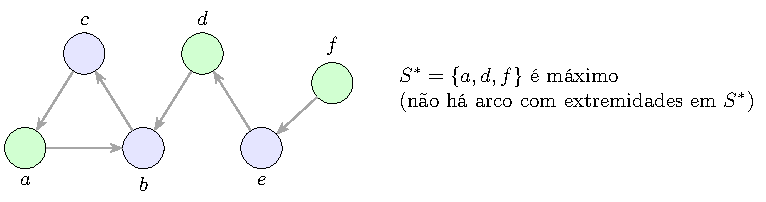
\includegraphics[width=0.9\linewidth]{figures/fig_empacotamento_max.pdf}

	\caption{Empacotamento máximo de vértices: para este digrafo, $S^{*}$ é um conjunto independente de maior cardinalidade.}
	\label{fig:empacotamento-max}
\end{figure}



Esses conceitos de conectividade e empacotamento de vértices nos levam a explorar as subestruturas especiais que existem em digrafos, que são similares às que vimos em grafos comuns, mas com algumas diferenças importantes devido à direção dos arcos.

\subsection{Subestruturas em digrafos}


Tal qual os grafos que discutimos na sessão anterior, os digrafos também possuem as mesmas estruturas especiais, essas estruturas chamadas sub-digrafos mudam um pouco em nomenclatura: caminhos quando direcionados são chamados de trilhas, e ciclos são chamados de circuitos e componentes conexas são componentes fortemente conexas e árvores viram arborescências. Além da nomenclatura, a direção dos arcos traz algumas nuances importantes, discutiremos sobre essas nuances apenas na sessão de arborescências e como os algoritmos de busca mudam bastante em complexidade se estamos tratando de arborescências ou árvores comuns.


Um \textbf{subdigrafo} \(D' = (V', A')\) de um digrafo \(D = (V, A)\) é um digrafo onde \(V' \subseteq V\) e \(A' \subseteq A\). Ou seja, \(D'\) é formado por um subconjunto dos vértices e arcos de \(D\).


\begin{figure}[H]
	\centering
	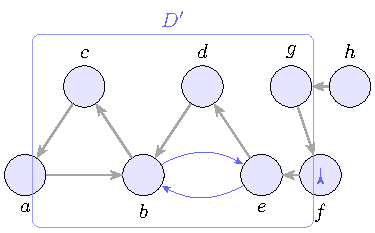
\includegraphics[width=0.9\linewidth]{figures/fig_subdigrafo.pdf}

	\caption{Subdigrafo: o subdigrafo $D'=(V',A')$ está destacado em azul. Aqui, $V'=\{b,c,d,e\}$ e $A'$ contém apenas arcos entre esses vértices.}
	\label{fig:subdigrafo}
\end{figure}


\subsubsection{Subdigrafos Induzidos}

Um subdigrafo pode ser \emph{induzido} por um conjunto de vértices \(V' \subseteq V\), denotado como \(D[V']\). Nesse caso, o conjunto de arcos \(A'\) inclui todos os arcos em \(A\) que têm ambas as extremidades em \(V'\), ou seja, \(A' = \{(u, v) \in A \mid u, v \in V'\}\).


\begin{figure}[H]
	\centering
	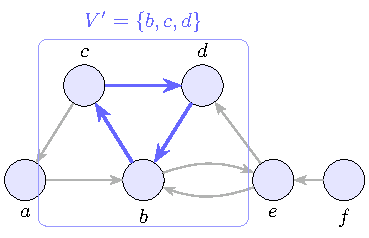
\includegraphics[width=0.9\linewidth]{figures/fig_subdigrafo_induzido.pdf}

	\caption{Subdigrafo induzido: para $V'=\{b,c,d\}$, $D[V']$ mantém todos os arcos com ambas as extremidades em $V'$.}
	\label{fig:subdigrafo-induzido}
\end{figure}


\subsubsection{Subdigrafo Maximal}

Um subdigrafo é tido como maximal se não é possível adicionar mais vértices ou arcos a ele sem perder alguma propriedade específica, como conexidade ou aciclicidade.


\begin{figure}[H]
	\centering
	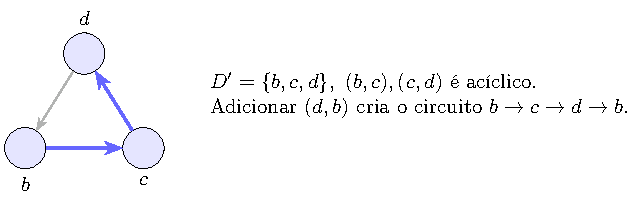
\includegraphics[width=0.9\linewidth]{figures/fig_subdigrafo_maximal.pdf}

	\caption{Subdigrafo maximal (por aciclicidade): $D'$ é acíclico e maximal em $D$; adicionar o arco restante $(d,b)$ cria um circuito.}
	\label{fig:subdigrafo-maximal}\end{figure}


\subsubsection{Subdigrafo Gerador}

Um subdigrafo é tido como gerador se inclui todos os vértices do digrafo original, ou seja, \(V' = V\). Nesse caso, o subdigrafo é formado por um subconjunto dos arcos do digrafo original.


\begin{figure}[H]
	\centering
	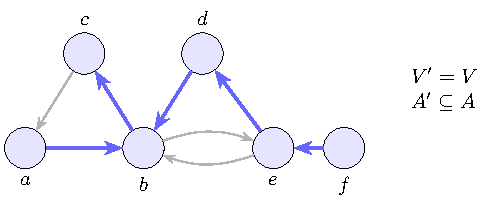
\includegraphics[width=0.9\linewidth]{figures/fig_subdigrafo_gerador.pdf}

	\caption{Subdigrafo gerador: inclui todos os vértices do digrafo original ($V'=V$) e apenas um subconjunto dos arcos (em azul).}
	\label{fig:subdigrafo-gerador}\end{figure}



Com essas definições em mente, podemos explorar as subdigrafos específicos que citaremos ao longo da dissertação, começando pelas trilhas, circuitos, componentes fortemente conexas, componentes-fonte e arborescências.

\subsection{Subdigrafos Especiais}

\subsubsection{Trilhas}


Uma \textbf{trilha} (ou caminho direcionado) em um digrafo é uma sequência de vértices conectados por arcos que respeitam a direção. Formalmente, uma trilha \(P\) de comprimento \(k \geq 1\) é uma sequência de vértices \(P = (v_1, v_2, \ldots, v_{k+1})\) tal que cada par consecutivo \((v_i, v_{i+1})\) é um arco em \(A\). O comprimento da trilha é o número de arcos que ela contém, que é \(k\).


\begin{figure}[H]
	\centering
	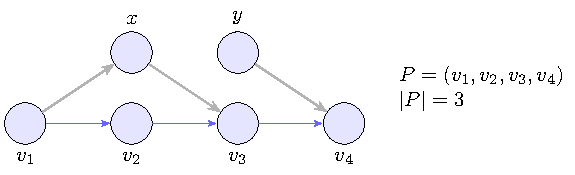
\includegraphics[width=0.9\linewidth]{figures/fig_trilha.pdf}

	\caption{Trilha em digrafo: a trilha $P=(v_1,v_2,v_3,v_4)$ está destacada em azul. Seu comprimento é o número de arcos percorridos, $|P|=3$.}
	\label{fig:trilha}\end{figure}



Uma conceito importante relacionado às trilhas é o de cortes.

\subsubsection{Cortes e Min-cortes}

Um \textbf{corte} em um digrafo é um conjunto de arcos cuja remoção desconecta o digrafo, ou seja, impede que haja uma trilha entre certos pares de vértices. Formalmente, dado um digrafo \(D = (V, A)\), um corte \(C\) é um subconjunto de arcos \(C \subseteq A\) tal que a remoção dos arcos em \(C\) resulta em um digrafo \(D' = (V, A \setminus C)\) onde não existe mais uma trilha (caminho direcionado) entre pelo menos um par de vértices \(u, v \in V\).


\begin{figure}[H]
	\centering
	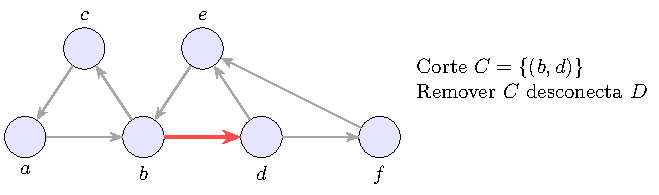
\includegraphics[width=0.9\linewidth]{figures/fig_corte.pdf}

	\caption{Corte em digrafo: o corte $C=\{(b,d)\}$ remove conectividade de $b$ para $d$.}
	\label{fig:corte}
\end{figure}



De forma resumida, dado um digrafo \(D=(V,A)\) e um subconjunto \(X\subseteq V\), denotamos por um corte \(s\text{--}t\) é determinado pela escolha de um conjunto de vértices \(X\subseteq V\) tal que \(s\in X\) e \(t\notin X\); pensa-se nele como a “divisão” do grafo em dois lados: \(X\) e \(V\setminus X\).

Para tornar a notação precisa e fácil de ler:
\begin{itemize}
	\item \textbf{\(s\text{--}t\)}: lê-se “de \(s\) para \(t\)”. Aqui, \(s\) é a fonte (onde o fluxo nasce) e \(t\) é o sumidouro (onde o fluxo chega).
	\item \textbf{\(\delta^+(X)\)} (fronteira de saída de \(X\)): conjunto de todos os arcos que \emph{saem} de \(X\) para fora, isto é, para \(V\setminus X\).
	\item \textbf{\(\delta^-(X)\)} (fronteira de entrada de \(X\)): conjunto de todos os arcos que \emph{entram} em \(X\) vindos de \(V\setminus X\). Note que \(\delta^-(X)=\delta^+(V\setminus X)\).
	\item \textbf{Valor do corte}: dado um peso (ou custo) \(c:A\to\mathbb{R}_+\) para cada arco, o valor do corte induzido por \(X\) é a soma dos pesos dos arcos que cruzam de \(X\) para fora:
	      \[c(\delta^+(X))=\sum_{a\in\delta^+(X)} c(a).\]
	      No caso não ponderado, esse valor coincide com a \emph{quantidade} de arcos que saem de \(X\).
\end{itemize}

\subsubsection{Exemplo:} se \(\delta^+(X)=\{(u_1,v_1),(u_2,v_2)\}\) com \(c((u_1,v_1))=2\) e \(c((u_2,v_2))=3\), então \(c(\delta^+(X))=2+3=5\).


Um min-corte é um corte de tamanho mínimo, ou seja, é o corte com o menor número possível de arcos cuja remoção desconecta o digrafo. Formalmente, dado um digrafo \(D = (V, A)\), um min-corte \(C_{min}\) é um corte tal que para qualquer outro corte \(C\), \(|C_{min}| \leq |C|\). O tamanho do min-corte é o número de arcos em \(C_{min}\).


\begin{figure}[H]
	\centering
	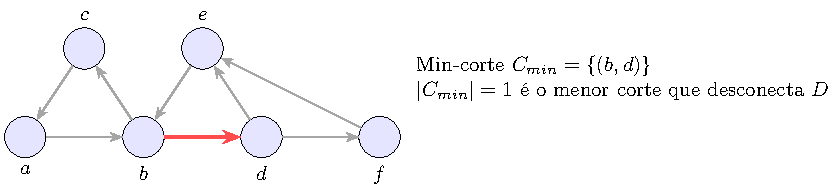
\includegraphics[width=0.9\linewidth]{figures/fig_min_corte.pdf}

	\caption{Min-corte em digrafo: o min-corte $C_{min}$ é um corte de menor cardinalidade (ou custo) que separa $s$ de $t$.}
	\label{fig:min-corte}
\end{figure}


Um teorema importante relacionado a min-cortes é o Teorema do Fluxo Máximo - Corte Mínimo, que estabelece uma relação entre o fluxo máximo que pode ser enviado de uma fonte \(s\) para um sumidouro \(t\) em um digrafo e o valor do min-corte que separa \(s\) de \(t\). Escolhemos apresensentar esse teorema aqui pois ele traz uma intuição interessante sobre a relação entre fluxos e cortes em digrafos, relevantes para os algoritmos que discutiremos mais adiante.


\begin{teobox}{Fluxo–Corte Máximo = Mínimo Corte.}{fluxo-corte}
	Em digrafos com limites/pesos não negativos nos arcos, o valor de um fluxo máximo de \(s\) para \(t\) é igual ao valor de um min-corte \(s\text{--}t\). Em símbolos: \(\max\,\text{valor}(f) = \min\, c(\delta^+(X))\), onde o mínimo é sobre \(X\subseteq V\) com \(s\in X\), \(t\notin X\), e \(c(\delta^+(X))=\sum_{a\in\delta^+(X)} c(a)\).

	\textbf{Prova (esboço):}

	\emph{(i) Desigualdade \(\le\).} Seja \(f\) um fluxo qualquer. Para um corte \((X, V\setminus X)\) com \(s\in X\), \(t\notin X\), a conservação de fluxo implica que o fluxo líquido que sai de \(X\) é exatamente \(\text{valor}(f)\).

	Logo, \[\text{valor}(f)= \sum_{a\in\delta^+(X)} f(a) - \sum_{a\in\delta^-(X)} f(a) \le \sum_{a\in\delta^+(X)} f(a) \le \sum_{a\in\delta^+(X)} c(a)=c(\delta^+(X)),\]

	pois \(f(a)\le c(a)\) para todo arco (limite). Como isso vale para todo \(X\), obtemos \(\text{valor}(f)\le \min_X c(\delta^+(X))\).


	\emph{(ii) Desigualdade \(\ge\) e igualdade.} Considere um fluxo máximo \(f\) sem caminho aumentante no \emph{grafo residual} \(R_f\) (isto é, não há como aumentar o valor do fluxo). Defina \(X\) como o conjunto de vértices alcançáveis a partir de \(s\) em \(R_f\). Então, não existe arco residual de \(X\) para \(V\setminus X\); logo, todo arco original que sai de \(X\) está saturado (\(f(a)=c(a)\)), e todo arco que entra em \(X\) carrega fluxo zero. Assim,

	\[\text{valor}(f)=\sum_{a\in\delta^+(X)} f(a)=\sum_{a\in\delta^+(X)} c(a)=c(\delta^+(X)).\]
	Portanto, \(f\) atinge exatamente o valor de um corte \(s\text{--}t\); em particular, esse corte é mínimo e \(f\) é máximo. \hfill$\square$


	\smallskip
	\textbf{Comentário:} Esse resultado é um protótipo de teorema \emph{min--max}: “empacotar” muito fluxo (caminhos) equivale a “cobrir” pouco com um corte. Ver, por exemplo, \cite{schrijver2003comb}.
\end{teobox}


Quando falamos em trilhas, precisamos também falar sobre circuitos, que são ciclos direcionados.
A diferença entre trilhas e circuitos é que trilhas são caminhos direcionados que não necessariamente retornam ao ponto de origem, enquanto circuitos são caminhos direcionados que começam e terminam no mesmo vértice.

\subsubsection{Circuitos}

Um \textbf{circuito} é um caminho direcionado que começa e termina no mesmo vértice, ou seja, \(v_1 = v_{k+1}\). Formalmente, um circuito \(C\) é uma sequência de vértices \(C = (v_1, v_2, \ldots, v_k, v_1)\) tal que cada par consecutivo \((v_i, v_{i+1})\) é um arco em \(A\) e \(k \geq 2\). O comprimento do circuito é o número de arcos que ele contém, que é \(k\).


\begin{figure}[H]
	\centering
	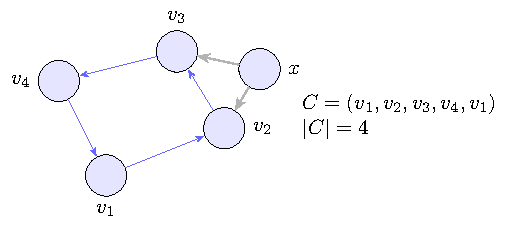
\includegraphics[width=0.9\linewidth]{figures/fig_ciclo_direcionado.pdf}

	\caption{Ciclo direcionado em digrafo: o ciclo $C=(v_1,v_2,v_3,v_4,v_1)$ está destacado em azul. Seu comprimento é o número de arcos, $|C|=4$.}
	\label{fig:ciclo-direcionado}\end{figure}



Propriedades importantes dos circuitos incluem:
\begin{itemize}
	\item \textbf{Circuito simples}: um circuito é dito simples se não repete vértices, exceto o vértice inicial/final. Ou seja, \(v_i \neq v_j\) para \(1 \leq i < j \leq k\).
	\item \textbf{Circuito Euleriano}: um circuito que percorre cada arco exatamente uma vez. Um digrafo possui um circuito euleriano se e somente se é fortemente conexo e o grau de entrada é igual ao grau de saída para cada vértice.
	\item \textbf{Circuito Hamiltoniano}: um circuito que visita cada vértice exatamente uma vez, exceto o vértice inicial/final. Determinar a existência de um circuito hamiltoniano é um problema que chamamos de NP-completo. Vamos explicar mais sobre isso na seção de algoritmos e complexidade computacional.
\end{itemize}


Existe um princípio chamado de princípio da casa dos pombos, que diz que se você tem mais pombos do que casas, pelo menos uma casa deve conter mais de um pombo. Em termos de grafos, isso se traduz na ideia de que se um grafo tem mais arestas do que vértices, ele deve conter pelo menos um ciclo.


Esse princípio também se aplica a digrafos, mas com uma nuance importante: em digrafos, o critério correto para garantir a existência de um circuito dirigido é que o grau mínimo de saída (ou de entrada) seja pelo menos 1. Ou seja, se cada vértice em um digrafo tem pelo menos um arco saindo dele (ou entrando nele), então o digrafo deve conter pelo menos um circuito dirigido. Abaixo apresentamos esse resultado formalmente.


\begin{lemabox}{Princípio da casa dos pombos para circuitos.}{casa-dos-pombos}
	Se \(D=(V,A)\) é um digrafo finito em que todo vértice tem grau de saída ao menos 1, isto é, \(d^+(v)\ge 1\) para todo \(v\in V\), então \(D\) contém pelo menos um circuito dirigido. (De forma equivalente, a afirmação vale trocando ``saída'' por ``entrada''.)


	\textbf{Prova:} Escolha para cada \(v\in V\) um arco \((v,f(v))\) que sai de \(v\) (possível porque \(d^+(v)\ge 1\)). Fixa\-do um vértice \(v_0\), considere a sequência \(v_0, v_1=f(v_0), v_2=f(v_1),\dots\). Como \(V\) é finito, algum vértice repete: existem \(i<j\) com \(v_i=v_j\). O trecho \(v_i\to v_{i+1}\to\cdots\to v_j=v_i\) é um circuito dirigido em \(D\). A versão com graus de entrada segue aplicando o argumento ao digrafo com arcos invertidos. \hfill$\square$


	\smallskip
	\textbf{Observação:} A condição \(|A|>|V|\) \emph{não} garante a existência de circuito dirigido em geral (há orientações acíclicas com muitos arcos). O critério correto, simples e útil, é o grau mínimo de saída (ou de entrada) ser pelo menos 1. Ver, por exemplo, \cite{schrijver2003comb}.

\end{lemabox}


Esse princípio ajuda a entender o comportamento básico dos métodos que os algoritmos empregam para encontrar as arborescências de custo mínimo. Vamos elaborar melhor esse ponto na seção de algoritmos em arborescências, especialmente ao discutir o algoritmo de Chu--Liu/Edmonds.


No algoritmo de Chu--Liu/Edmonds que exploraremos em detalhes em capítulo posterior, para cada vértice \(v\neq r\), escolhemos a aresta de menor custo que entra em \(v\), o subgrafo obtido fica com grau de entrada igual a 1 em todos os \(v\neq r\). Pelo lema, enquanto esse subgrafo ainda não for uma arborescência, ele necessariamente contém um circuito: assim o algoritmo se baseia em detectar o circuitos, contraí-lo a um único vértice e repetir a seleção sob custos reduzidos. Quando não houver mais circuitos, as arestas escolhidas formam uma arborescência ótima enraizada em \(r\).

\subsubsection{Componentes fortemente conexas}
Uma \textbf{componente fortemente conexa} (abreviaremos como \textbf{CFC}) é um subdigrafo maximal onde existe um caminho direcionado (trilha) entre qualquer par de vértices.


Formalmente, uma componente fortemente conexa \(C\) é um subdigrafo \(C = (V_C, A_C)\) onde \(V_C \subseteq V\) e \(A_C \subseteq A\), que satisfaz a seguinte propriedade:
\begin{itemize}
	\item \(C\) é fortemente conexo: existe um caminho direcionado entre qualquer par de vértices em \(V_C\).
\end{itemize}
Além disso, \(C\) é maximal, o que significa que não é possível adicionar mais vértices ou arcos a \(C\) sem perder a propriedade de forte conexidade.

\begin{figure}[H]
	\centering
	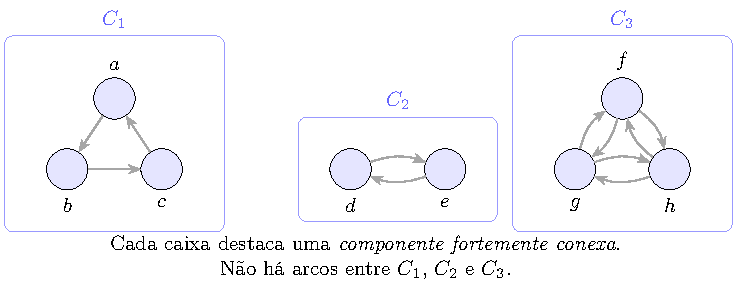
\includegraphics[width=0.9\linewidth]{figures/figure_028.pdf}

	\caption{Componentes fortemente conexas: o digrafo possui três componentes $C_1$, $C_2$ e $C_3$. Cada $C_i$ é fortemente conexo e \emph{maximal}.}
\end{figure}



A seguir falaremos sobre a propriedade de alcançabilidade mútua em CFC, que é fundamental para entendermos a relação entre elas e arborescências (que apenas mencionaremos aqui, para aprofundarmos na sessão sobre arborescências e com os grafos acíclicos dirigidos (DAGs))\footnote{Um DAG (Directed Acyclic Graph) é um grafo direcionado que não contém ciclos. Em outras palavras, não é possível começar em um vértice e seguir uma sequência de arcos que retorne ao mesmo vértice. Os DAGs são estruturas fundamentais em muitas áreas da computação, incluindo a representação de dependências e a modelagem de processos.}:

\begin{itemize}
	\item \textbf{CFCs e alcançabilidade mútua:} dois vértices \(u\) e \(v\) pertencem à mesma CFC se, e somente se, \(u\leadsto v\) e \(v\leadsto u\). Ou seja, existe um caminho direcionado de \(u\) para \(v\) e um caminho direcionado de \(v\) para \(u\). A relação de pertencer à mesma CFC é uma relação de equivalência que particiona o conjunto de vértices \(V\) em subconjuntos disjuntos, cada um correspondendo a uma CFC.
	\item \textbf{Arborescências em digrafos fortemente conexos:} um digrafo é fortemente conexo se, e somente se, para algum (equiv., para todo) vértice $r$ existem uma \emph{arborescência de saída} enraizada em $r$ que alcança todos os vértices e uma \emph{arborescência de entrada} enraizada em $r$ que é alcançada por todos os vértices. De fato, se $D$ é fortemente conexo, basta rodar buscas a partir de $r$; no sentido inverso, $r\leadsto v$ pela arborescência de saída e $v\leadsto r$ pela de entrada, implicando alcançabilidade mútua entre quaisquer dois vértices via $r$.
	\item \textbf{CFC e DAG.} Ao \emph{contrair} cada CFC a um único vértice obtemos o grafo condensado $\mathrm{Cond}(D)$\footnote{O grafo condensado é uma representação simplificada do digrafo original, onde as CFCs são representadas como vértices únicos.}. Não há circuitos dirigidos em $\mathrm{Cond}(D)$; portanto, ele é um DAG.

	      \subsubsection{Consequências:}
	      todo DAG tem ao menos uma componente-fonte (falaremos em seguida sobre eles) e uma componente-sumidouro; logo, $\mathrm{Cond}(D)$ também tem ao menos uma CFC-fonte e ao menos uma CFC-sumidouro.
\end{itemize}

\subsubsection{Componentes-fonte}
Uma \textbf{componente-fonte} é uma componente fortemente conexa que não possui arcos direcionados saindo dela para outras componentes. Formalmente, uma componente-fonte \(C\) é uma componente fortemente conexa \(C = (V_C, A_C)\) onde \(V_C \subseteq V\) e \(A_C \subseteq A\), que satisfaz a seguinte propriedade:
\begin{itemize}
	\item Não existem arcos \((u, v) \in A\) tais que \(u \in V_C\) e \(v \notin V_C\).
	\item \(C\) é maximal: não é possível adicionar mais vértices ou arcos a \(C\) sem perder a propriedade de forte conexidade.
	\item \(C\) é fortemente conexo: existe um caminho direcionado entre qualquer par de vértices em \(V_C\).
\end{itemize}


\begin{figure}[H]
	\centering
	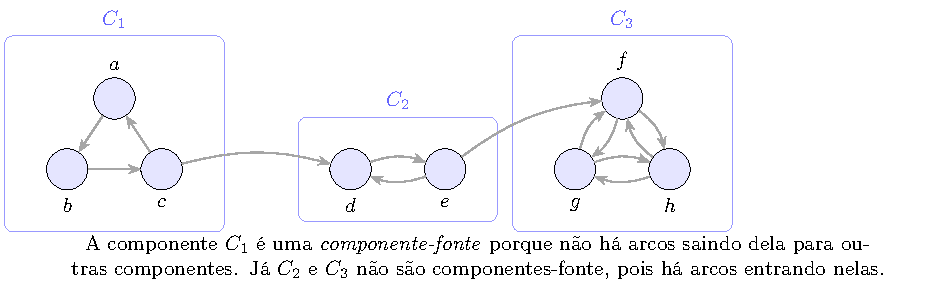
\includegraphics[width=0.9\linewidth]{figures/fig_componente_fonte.pdf}

	\caption{Componente-fonte: o digrafo possui três componentes $C_1$, $C_2$ e $C_3$. A componente $C_1$ é uma componente-fonte porque não há arcos saindo dela para outras componentes. Já $C_2$ e $C_3$ não são componentes-fonte, pois há ar  cos entrando nelas.}
	\label{fig:componente-fonte}\end{figure}


\subsubsection{Componentes-sumidouro}
Uma \textbf{componente-sumidouro} é uma componente fortemente conexa que não possui arcos direcionados entrando nela vindos de outras componentes. Formalmente, uma componente-sumidouro \(C\) é uma componente fortemente conexa \(C = (V_C, A_C)\) onde \(V_C \subseteq V\) e \(A_C \subseteq A\), que satisfaz a seguinte propriedade:
\begin{itemize}
	\item Não existem arcos \((u, v) \in A\) tais que \(u \notin V_C\) e \(v \in V_C\).
	\item \(C\) é maximal: não é possível adicionar mais vértices ou arcos a \(C\) sem perder a propriedade de forte conexidade.
	\item \(C\) é fortemente conexo: existe um caminho direcionado entre qualquer par de vértices em \(V_C\).
\end{itemize}


\begin{figure}[H]
	\centering
	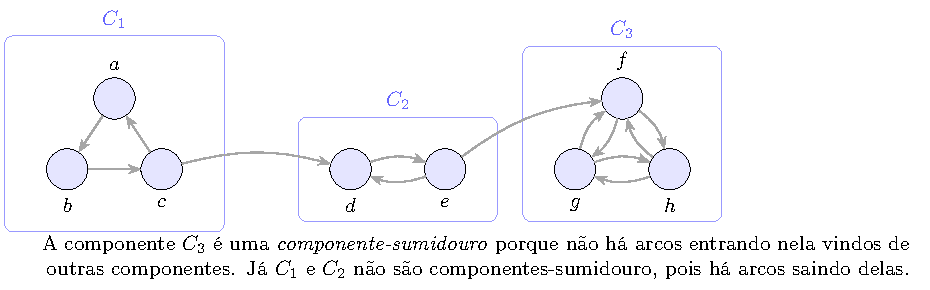
\includegraphics[width=0.9\linewidth]{figures/fig_componente_sumidouro.pdf}

	\caption{Componente-sumidouro: o digrafo possui três componentes $C_1$, $C_2$ e $C_3$. A componente $C_3$ é uma componente-sumidouro porque não há arcos entrando nela vindos de outras componentes. Já $C_1$ e $C_2$ não são componentes-sumidouro, pois há arcos saindo delas.}
	\label{fig:componente-sumidouro}\end{figure}



Existe um resultado clássico que relaciona o número de componentes-fonte e componentes-sumidouro em um digrafo com o número mínimo de arcos necessários para torná-lo fortemente conexo.


\begin{figure}[H]
	\centering
	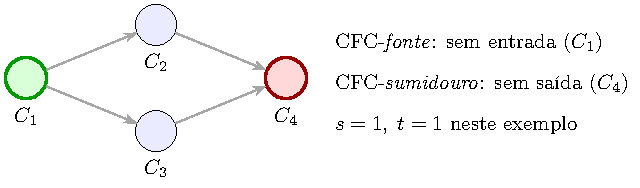
\includegraphics[width=0.9\linewidth]{figures/fig_condensado_st.pdf}

	\caption{Grafo condensado $\mathrm{Cond}(D)$: cada CFC é contraída a um vértice e não há circuitos dirigidos (DAG).}
	\label{fig:condensado-st}
\end{figure}



Seja $D=(V,A)$ um digrafo com $k$ componentes fortemente conexas (CFCs):


Denote por $\mathrm{Cond}(D)$ o grafo \emph{condensado}, obtido ao contrair cada CFC de $D$ em um único vértice; $\mathrm{Cond}(D)$ é sempre um DAG. Escreva $s$ para o número de CFCs-\emph{fonte} (vértices de $\mathrm{Cond}(D)$ sem arcos de \emph{entrada}) e $t$ para o número de CFCs-\emph{sumidouro} (vértices de $\mathrm{Cond}(D)$ sem arcos de \emph{saída}). Com essa notação, vale o seguinte:


\begin{lemabox}{Mínimo de arcos para conexidade forte}{min-arc}
	Se $k=1$, então $D$ já é fortemente conexo e o mínimo de arcos a adicionar é $0$. Se $k\ge 2$, o número mínimo de arcos a adicionar para tornar $D$ fortemente conexo é \[\boxed{\;\max\{s,\,t\}\;}\,.\]


	\textbf{Prova (esboço).}

	\emph{Necessidade:} em qualquer supergrafo fortemente conexo, cada CFC-fonte deve receber ao menos um arco \emph{entrando} e cada CFC-sumidouro deve ter ao menos um arco \emph{saindo}; logo, são necessários ao menos $\max\{s,t\}$ arcos novos.


	\emph{Suficiência:} numa ordenação topológica de $\mathrm{Cond}(D)$, conecte CFCs-sumidouro a CFCs-fonte de modo a formar um ciclo que percorra todas as CFCs. Isso pode ser feito com exatamente $\max\{s,t\}$ arcos, mesmo quando $s\ne t$, emparelhando sobras de um lado com o outro.


	Ver, por exemplo, textos clássicos sobre digrafos (e.g., \cite{schrijver2003comb}).
\end{lemabox}


Esse lema explica por que todo digrafo com mais de uma CFC-fonte ou mais de uma CFC-sumidouro não pode ser fortemente conexo. Além disso, ele é útil em algoritmos que buscam tornar um digrafo fortemente conexo, pois fornece um limite inferior para o número de arcos que precisam ser adicionados.


As noções de CFCs e componentes-fonte conversam diretamente com o conceito de \emph{arborescências}. Pois, em uma arborescência, todos os vértices são alcançáveis a partir da raiz, o que não implica que a arborescência é fortemente conexa, mas encontrar essas componentes dentro de um digrafo pode nos ajudar em uma busca otimizada por arborescências.

\subsubsection{Arborescências}

Uma \textbf{arborescência} é um digrafo acíclico e conexo, onde há um vértice especial chamado \emph{raiz} que tem um caminho direcionado para todos os outros vértices. Formalmente, uma arborescência \(T\) é um digrafo \(T = (V_T, A_T)\) onde \(V_T \subseteq V\) e \(A_T \subseteq A\), tal que \(T\) é conexo (existe um caminho direcionado da raiz para qualquer vértice em \(V_T\)) e \(T\) é acíclico (não contém ciclos direcionados). Além disso, uma arborescência com \(n\) vértices sempre tem exatamente \(n-1\) arcos.

\begin{figure}[H]
	\centering
	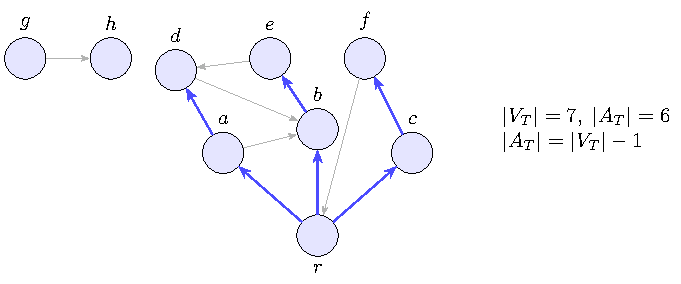
\includegraphics[width=0.9\linewidth]{figures/fig_arborescencia.pdf}

	\caption{Arborescência: digrafo conexo e acíclico com raiz $r$ de onde há um caminho direcionado para todos os outros vértices em azul. No exemplo, $|V_T|=7$ e $|A_T|=6$, satisfazendo $|A_T|=|V_T|-1$. Em cinza, arcos que não fazem parte da arborescência.}
	\label{fig:arborescencia}\end{figure}


\subsubsection{Definições e notação adicionais}

Para facilitar a discussão sobre arborescências, introduzimos algumas definições e notações adicionais: seja \(D = (V, A)\) um digrafo e \(r \in V\) um vértice específico (a raiz). Denotamos por \(d_D^+(v)\) o grau de saída de um vértice \(v\) em \(D\), ou seja, o número de arcos que saem de \(v\). Analogamente, \(d_D^-(v)\) é o grau de entrada de \(v\), o número de arcos que entram em \(v\).



As arborescências são o principal objeto de investigação desse trabalho, portanto vamos usar uma sessão dedicada a elas para apresentar suas características, variações e aplicações.

\section{Arborescências em foco}


Já tratamos do conceito básico de arborescência, agora falaremos de arborescências especiais:

\subsection{Arborescência Geradora}
Uma arborescência é considerada geradora se inclui todos os vértices do digrafo original, ou seja, \(V_T = V\). Nesse caso, a arborescência é formada por um subconjunto dos arcos do digrafo original.

\subsection{Arborescência Maximal}
Uma arborescência é dita maximal se não é possível adicionar mais vértices ou arcos a ela sem perder a propriedade de ser uma arborescência, ou seja, sem criar ciclos ou desconectar o digrafo.

\subsection{Ramificações Geradoras}
Uma \textbf{ramificação geradora} é um subdigrafo que é uma arborescência que inclui todos os vértices do digrafo original. Formalmente, uma ramificação geradora \(R\) é um subdigrafo \(R = (V_R, A_R)\) onde \(V_R = V\) e \(A_R \subseteq A\), que satisfaz as seguintes propriedades: \(R\) é uma arborescência (existe um vértice especial chamado raiz que tem um caminho direcionado para todos os outros vértices) e \(R\) é maximal (não é possível adicionar mais arcos a \(R\) sem perder a propriedade de ser uma arborescência).


\begin{figure}[H]
	\centering
	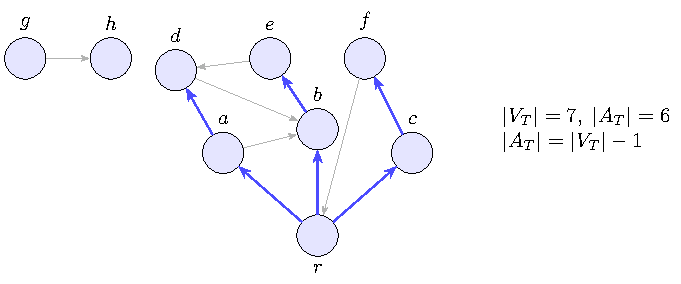
\includegraphics[width=0.9\linewidth]{figures/fig_ramificacao_geradora.pdf}

	\caption{Ramificação geradora: arborescência que inclui todos os vértices do digrafo original, em azul. No exemplo, $|V_T|=7$ e $|A_T|=6$, satisfazendo $|A_T|=|V_T|-1$. Em cinza, arcos que não fazem parte da ramificação geradora.}
	\label{fig:ramificacao-geradora}\end{figure}



Quando falamaos de ramificações geradoras, podemos falar de uma estrutura que fixa um vértice raiz \(r\) e constrói uma arborescência que alcança todos os outros vértices a partir dessa raiz. Essa estrutura é conhecida como \emph{r-arborescência}.

\subsection{Arborescência de Raiz Específica}
Uma arborescência de raiz específica é uma arborescência onde a raiz é um vértice pré-determinado do digrafo. Isso é útil em situações onde um ponto de origem específico deve ser o início dos caminhos direcionados para todos os outros vértices. Podemos chamá-la de r-arborescência, onde \(r\) é o vértice raiz.


Em uma arborescência \(T = (V_T, A_T)\) enraizada em \(r\), temos as seguintes propriedades: a raiz \(r\) tem grau de entrada zero (\(d_T^-(r) = 0\)); todo outro vértice \(v \in V_T \setminus \{r\}\) tem grau de entrada exatamente um (\(d_T^-(v) = 1\)), o que significa que há exatamente um arco direcionado entrando em cada vértice, exceto na raiz; o grau de saída \(d_T^+(v)\) pode variar, mas para garantir que \(T\) seja conexo, deve haver pelo menos um arco saindo de \(r\) para alcançar os outros vértices.\subsection{Arborescência inversa (in-arborescência)}
uma \emph{arborescência inversa} enraizada em \(r\) — também chamada de \emph{in-arborescência} — é o resultado de inverter a orientação de todos os arcos de uma arborescência (out-arborescência) enraizada em \(r\). Equivalentemente: é um digrafo acíclico no qual, para todo \(v\neq r\), existe \emph{exatamente um} caminho direcionado de \(v\) até \(r\) (isto é, todos os arcos estão orientados \emph{em direção} à raiz). Em termos de graus, numa in-arborescência cada vértice \(v\neq r\) tem grau de saída igual a 1 (o arco para seu “pai”) e a raiz \(r\) tem grau de saída 0; os graus de entrada são complementares aos de uma out-arborescência.


As arborecências podem ter custos associados aos seus arcos, o que nos leva ao conceito de arborescência de custo mínimo.

\subsection{Arborescência de Custo Mínimo}

Uma \textbf{arborescência de custo mínimo} é uma arborescência que minimiza a soma dos pesos dos arcos que a compõem. Esse conceito é especialmente relevante em aplicações onde os arcos têm custos associados, como em redes de transporte ou comunicação.


Finalmente podemos conceituar a principal estrutura que estudaremos nesta dissertação: a r-arborescência de custo mínimo e sua variante, a r-arborescência inversa de custo mínimo.

\subsection{r-arborescência de custo mínimo}
é uma arborescência enraizada em um vértice específico \(r\) que minimiza a soma dos pesos dos arcos que a compõem. Formalmente, dada uma função de custo \(c: A \to \mathbb{R}_{\geq 0}\) que atribui um custo a cada arco do digrafo \(D = (V, A)\), uma r-arborescência de custo mínimo \(T\) é uma arborescência \(T = (V_T, A_T)\) onde \(V_T \subseteq V\) e \(A_T \subseteq A\), tal que \(T\) é uma arborescência enraizada em \(r\) (existe um caminho direcionado de \(r\) para qualquer vértice em \(V_T\)) e \(T\) minimiza o custo total (a soma dos custos dos arcos em \(A_T\) é mínima, ou seja, \(\sum_{a \in A_T} c(a)\) é minimizada).\begin{figure}[H]
	\centering
	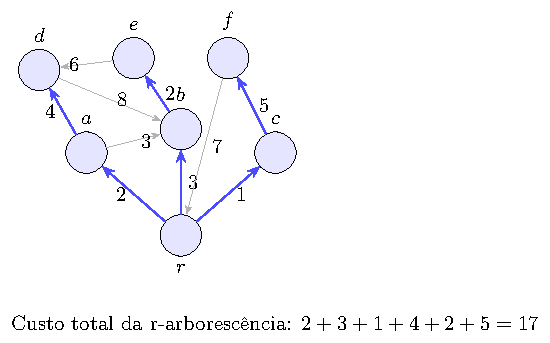
\includegraphics[width=0.9\linewidth]{figures/fig_r_arborescencia_custo_minimo.pdf}

	\caption{r-arborescência de custo mínimo: arborescência enraizada em $r$ que minimiza a soma dos custos dos arcos, em azul. No exemplo, o custo total é $17$. Em cinza, arcos que não fazem parte da r-arborescência de custo mínimo.}
	\label{fig:r-arborescencia-custo-minimo}\end{figure}


\subsection{r-arborescência inversa de custo mínimo}
é uma arborescência inversa enraizada em um vértice específico \(r\) que minimiza a soma dos pesos dos arcos que a compõem. Formalmente, dada uma função de custo \(c: A \to \mathbb{R}_{\geq 0}\) que atribui um custo a cada arco do digrafo \(D = (V, A)\), uma r-arborescência inversa de custo mínimo \(T\) é uma arborescência inversa \(T = (V_T, A_T)\) onde \(V_T \subseteq V\) e \(A_T \subseteq A\), tal que \(T\) é uma arborescência inversa enraizada em \(r\) (existe um caminho direcionado de qualquer vértice em \(V_T\) até \(r\)) e \(T\) minimiza o custo total (a soma dos custos dos arcos em \(A_T\) é mínima, ou seja, \(\sum_{a \in A_T} c(a)\) é minimizada).



\begin{figure}[H]
	\centering
	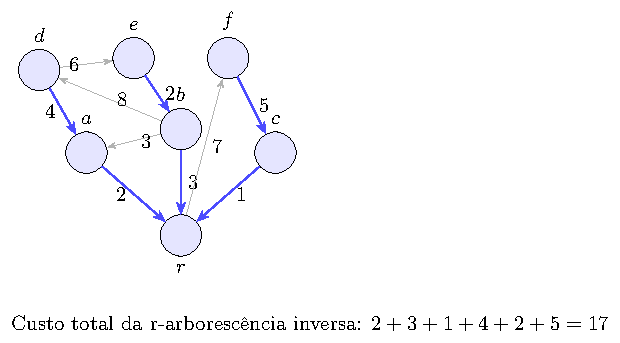
\includegraphics[width=0.9\linewidth]{figures/fig_r_arborescencia_inversa_custo_minimo.pdf}

	\caption{r-arborescência inversa de custo mínimo: arborescência inversa enraizada em $r$ que minimiza a soma dos custos dos arcos, em azul. No exemplo, o custo total é $17$. Em cinza, arcos que não fazem parte da r-arborescência inversa de custo mínimo.}
	\label{fig:r-arborescencia-inversa-custo-minimo}\end{figure}



As arborescências são a principal estrutura que exploraremos ao longo desta dissertação, especialmente a r-arborescência de custo mínimo e r-arborescência inversa de custo mínimo, abordaremos o problema de encontrá-las eficientemente em digrafos com custos associados aos arcos.



\subsection{Noções aprofundadas em arborescências}


Vamos explorar algumas propriedades e teoremas importantes relacionados a arborescências, que serão úteis para entender os algoritmos que discutiremos posteriormente.

\subsection{Grau e contagem de arcos}

Seja $T$ uma out-arborescência enraizada em $r$ com $n$ vértices. Ela é exatamente a estrutura que satisfaz as três condições combinadas abaixo (todas muito fáceis de checar):
\begin{enumerate}\setlength{\itemsep}{2pt}
	\item (Contagem) $|A_T| = n-1$.
	\item (Entrada única) Cada vértice $v\neq r$ recebe exatamente um arco: $d_T^-(v)=1$.
	\item (Raiz sem entrada) A raiz não recebe arcos: $d_T^-(r)=0$.
\end{enumerate}
De forma simétrica, numa in-arborescência (arborescência inversa) valem as versões “espelhadas”: cada $v\neq r$ tem exatamente um arco \emph{saindo} ($d_T^+(v)=1$) e a raiz tem grau de saída zero ($d_T^+(r)=0$).


Reciprocamente, qualquer subdigrafo que satisfaça (1)--(3) é uma out-arborescência enraizada em $r$ (e análogamente no caso inverso).

\subsection{Discussões importantes sobre arborescências}


Dado um digrafo \(D = (V, A)\) e um vértice raiz \(r \in V\), uma questão fundamental é determinar quando existe uma arborescência enraizada em \(r\).
Existem alguns resultados clássicos que caracterizam a existência de arborescências em digrafos, bem como condições para a existência de múltiplas arborescências disjuntas. Vamos apresentar dois teoremas fundamentais nesse contexto.

\subsection{Teorema de Fulkerson}


Existem várias formas de caracterizar a existência de arborescências em um digrafo. Uma delas é via a condição de cortes, que estabelece uma relação entre a existência de arborescências e a estrutura dos cortes no digrafo.


Esse resultado é conhecido como o \textbf{Teorema de Fulkerson} e para entendermos ele precisamos ter em mente as seguintes definições:

\begin{itemize}
	\item Seja \(D = (V, A)\) um digrafo e \(X \subseteq V\) um subconjunto de vértices. O conjunto \(\delta^-(X)\) é definido como o conjunto de todos os arcos que entram em \(X\) vindos de \(V \setminus X\). Formalmente,
	      \[
		      \delta^-(X) = \{(u, v) \in A : u \in V \setminus X, v \in X\}.
	      \]
	\item Um corte em um digrafo é uma partição dos vértices em dois subconjuntos disjuntos. O conjunto \(\delta^-(X)\) representa o corte que separa \(X\) do resto do grafo.
\end{itemize}


A seguir apresentamos o teorema propriamente dito e um esboço de sua prova.


\begin{teobox}{Condição de existência via cortes (Fulkerson)}{fulkerson-existencia}
	Seja $D=(V,A)$ e $r\in V$. Existe uma out-arborescência (arborescência dirigida) enraizada em $r$ se, e somente se,
	\[
		\forall\, X\subseteq V\setminus\{r\},\ X\neq\emptyset:\  \delta^-(X)\neq\emptyset.
	\]
	Isto é: todo subconjunto não vazio que não contém a raiz recebe ao menos um arco vindo de fora.


	\textbf{Prova (esboço):}


	\emph{(Só se:)} Suponha que $T$ é uma out-arborescência enraizada em $r$. Pegue qualquer $X\neq\emptyset$ sem $r$. Considere o primeiro vértice de $X$ alcançado a partir de $r$ no caminho dentro de $T$; o arco imediatamente anterior entra em $X$ e pertence a $\delta^-(X)$. Logo $\delta^-(X)\neq\emptyset$.


	\emph{(Se:)} Agora suponha que toda parte $X$ não vazia sem $r$ recebe um arco. Construímos $T$ iterativamente: comece com $S=\{r\}$. Enquanto $S\neq V$, tome um vértice $v\in V\setminus S$ tal que existe um arco $(u,v)$ com $u\in S$ (existe porque, caso contrário, o conjunto $X=V\setminus S$ não receberia arco). Adicione $v$ e o arco $(u,v)$. Não criamos ciclos porque cada novo vértice entra com exatamente um arco e só aponta para frente (a direção é de um vértice já inserido para um novo). Ao final, cada $v\neq r$ tem exatamente um arco de entrada e o grafo é conexo a partir de $r$, logo obtivemos uma out-arborescência.

	\medskip
	\textbf{Intuição curta.} A condição “todo $X$ tem um arco entrando” impede que qualquer bloco de vértices fique isolado da raiz; o processo guloso de anexar o primeiro arco que entra em cada bloco produz a arborescência sem retrocessos.

	\medskip
	\emph{Referência:} ver, por exemplo, \cite{schrijver2003comb}.
	\label{thm:fulkerson-cut-arborescencia}
\end{teobox}


Outro resultado clássico é o teorema que caracteriza a existência de múltiplas arborescências arcodisjuntas em um digrafo, conhecido como o \textbf{Teorema de Edmonds}. Precisamos de algumas definições antes de enunciá-lo:

\begin{itemize}
	\item Duas arborescências são ditas \emph{arcodisjuntas} se não compartilham nenhum arco, ou seja, \(A_{T_1} \cap A_{T_2} = \emptyset\).
	\item A condição de cortes para múltiplas arborescências estabelece que, para qualquer subconjunto \(X \subseteq V \setminus \{r\}\), o número de arcos que entram em \(X\) deve ser pelo menos igual ao número de arborescências desejadas.
	\item Uma out-arborescência enraizada em \(r\) é uma arborescência onde todos os caminhos direcionados partem de \(r\) e alcançam todos os outros vértices.
	\item O conjunto \(\delta^-(X)\) é definido como o conjunto de todos os arcos que entram em \(X\) vindos de \(V \setminus X\). Formalmente,
	      \[
		      \delta^-(X) = \{(u, v) \in A : u \in V \setminus X, v \in X\}.
	      \]
	\item Um corte em um digrafo é uma partição dos vértices em dois subconjuntos disjuntos. O conjunto \(\delta^-(X)\) representa o corte que separa \(X\) do resto do grafo.
\end{itemize}


Antes de enunciar o teorema, vale a pena mencionar o conceito de \emph{interseção de matroides}, mas, para não alongar demais, deixamos a explicação detalhada para o Apêndice \ref{ap:matroides}. Aqui, apenas uma breve introdução:
\begin{itemize}
	\item Matroides, são estruturas combinatórias que generalizam a noção de independência linear em álgebra linear. A interseção de matroides é um conceito que permite combinar duas ou mais estruturas de matroides para formar uma nova estrutura que mantém certas propriedades de independência.
	\item A interseção de matroides é frequentemente utilizada em problemas de otimização combinatória, onde é necessário encontrar soluções que satisfaçam múltiplas condições de independência simultaneamente.
	\item Familia de conjuntos independentes: cada matroide é definido por uma coleção de subconjuntos de um conjunto finito, chamados de conjuntos independentes, que satisfazem certas propriedades.
	\item No contexto de arborescências, a interseção de matroides pode ser usada para modelar a seleção de arcos que formam múltiplas arborescências arcodisjuntas, garantindo que cada arborescência mantenha suas propriedades de independência.
\end{itemize}



\begin{figure}[H]
	\centering
	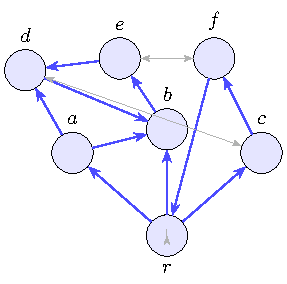
\includegraphics[width=0.9\linewidth]{figures/fig_exemplo_multiplas_arborescencias.pdf}

	\caption{digrafo de exemplo para múltiplas arborescências arcodisjuntas.}
	\label{fig:exemplo-multiplas-arborescencias}\end{figure}



Agora podemos enunciar o teorema de Edmonds, que fornece uma condição necessária e suficiente para a existência de \(k\) arborescências arcodisjuntas enraizadas em um vértice \(r\).


\begin{teobox}{$k$ arborescências arcodisjuntas (Edmonds)}{edmonds-k-arborescencias}
	Seja $D=(V,A)$, $r\in V$ e $k\ge 1$ inteiro. São equivalentes:
	\begin{enumerate}\setlength{\itemsep}{4pt}
		\item Existem $k$ out-arborescências enraizadas em $r$ que são par a par \emph{arcodisjuntas}.
		\item (Condição de cortes) Para todo subconjunto $X\subseteq V\setminus\{r\}$ vale $|\delta^-(X)| \ge k$.
	\end{enumerate}
	Em palavras: cada “bloco” $X$ que não contém a raiz precisa ter pelo menos $k$ arcos distintos chegando de fora; isso é exatamente o que permite ``alimentar'' $X$ a partir de $r$ em $k$ estruturas de ramificação independentes.


	\textbf{Prova (esboço):}
	\emph{(1 $\Rightarrow$ 2)} Se temos $k$ out-arborescências arcodisjuntas, então cada arborescência deve entrar em qualquer $X$ (senão não alcançaria seus vértices). Como os arcos são distintos entre as $k$ estruturas, precisamos de pelo menos $k$ arcos entrando em $X$; logo $|\delta^-(X)|\ge k$.


	\emph{(2 $\Rightarrow$ 1)} Trata-se a construção como um problema de \emph{interseção de matroides} ou aplicamos um procedimento incremental de troca (``\textit{augmenting}''). O conjunto de arcos pode suportar no máximo $k(n-1)$ arcos selecionados se quisermos $k$ arborescências, onde cada vértice $v \neq r$ recebe exatamente $k$ arcos de entrada (um de cada arborescência). A condição de cortes impede gargalos: se algum subconjunto $X$ tivesse menos que $k$ arcos entrando, seria impossível abastecer seus vértices com $k$ escolhas independentes.


	Uma prova clássica (Edmonds) formula o problema como interseção de duas famílias independentes:


	(i) uma família que limita a quantidade de arcos entrando em cada vértice a no máximo $k$;


	(ii) uma família que evita a criação de ciclos dirigidos ao selecionar arcos (estrutura de matroide de partição + matroide gráfico orientado).


	A hipótese de cortes garante que o algoritmo de aumento (que tenta adicionar um arco e, se criar ciclo ou saturar um vértice, realiza trocas) nunca fica travado antes de atingir $k(n-1)$ arcos. Agrupando, particionamos esses $k(n-1)$ arcos em $k$ coleções de $(n-1)$ arcos cada, que formam as $k$ out-arborescências arcodisjuntas.

	\medskip
	\emph{Referências:} Edmonds (teorema das branchings) \cite{edmonds1967optimum}, apresentações modernas em \cite{schrijver2003comb}.
	\label{thm:edmonds-disjoint-arborescencias}
\end{teobox}


Teoremas como esses servem para responder perguntas do tipo “quando existe?” e “quão rica pode ser a estrutura?”. Em particular, eles nos dizem que:
\begin{itemize}\setlength{\itemsep}{2pt}
	\item A existência de uma arborescência enraizada em \(r\) é garantida se, e somente se, todo subconjunto não vazio que não contém \(r\) recebe pelo menos um arco vindo de fora (Teorema de Fulkerson).
	\item A existência de \(k\) arborescências arcodisjuntas enraizadas em \(r\) é garantida se, e somente se, todo subconjunto não vazio que não contém \(r\) recebe pelo menos \(k\) arcos vindos de fora (Teorema de Edmonds).
\end{itemize}


Mas, agora estamos interessados em achar essas arborescências de forma eficiente, especialmente quando os arcos têm custos associados. Queremos encontrar a r-arborescência de custo mínimo, ou seja, a arborescência enraizada em \(r\) que minimiza a soma dos custos dos arcos que a compõem.


Um resultado central agora é a caracterização de \emph{optimalidade} para r-arborescências de custo mínimo: as chamadas \emph{condições de Fulkerson}. Elas conectam a solução primal (os arcos escolhidos) a um certificado dual (potenciais em subconjuntos) via custos reduzidos.

\subsubsection{Terminologia:}

Para um digrafo $D=(V,A)$, raiz $r$ e custos $c:A\to \mathbb{R}_{\ge 0}$, um subconjunto não vazio $X\subseteq V\setminus\{r\}$ é dito \textbf{apertado} (para uma família de pesos $y$) se exatamente um arco da solução escolhida entra em $X$ e $y(X)>0$.


Diremos que um arco $a=(u,v)$ \emph{entra} em $X$ se $u\notin X$ e $v\in X$.


Dada uma família de pesos $y: \{X\subseteq V\setminus\{r\}: X\neq\emptyset\}\to \mathbb{R}_{\ge 0}$, definimos o \textbf{custo reduzido} de $a$ por
\[
	c'(a) \;=\; c(a)\; - \sum_{\substack{X\subseteq V\setminus\{r\},\\ X\neq\emptyset,\ u\notin X,\ v\in X}} y(X).
\]


\begin{teobox}{Optimalidade de Fulkerson (r-arborescência de custo mínimo)}{fulkerson-opt}
	Seja $D=(V,A)$, raiz $r$ e custos $c:A\to\mathbb{R}_{\ge 0}$. Seja $T$ uma out-arborescência enraizada em $r$. As afirmações são equivalentes:
	\begin{enumerate}\setlength{\itemsep}{4pt}
		\item $T$ tem custo mínimo entre todas as out-arborescências enraizadas em $r$.
		\item Existem pesos $y(X)\ge 0$ para cada $\emptyset\neq X\subseteq V\setminus\{r\}$ tais que:
		      \begin{enumerate}\setlength{\itemsep}{2pt}
			      \item[(a)] $c'(a)\ge 0$ para todo arco $a\in A$ (não negatividade dos custos reduzidos);
			      \item[(b)] $c'(a)=0$ para todo arco $a\in T$ (complementaridade em arcos usados);
			      \item[(c)] Para todo $X$ com $y(X)>0$ entra \emph{exatamente um} arco de $T$ em $X$ (complementaridade em conjuntos apertados).
		      \end{enumerate}
	\end{enumerate}
	Além disso, quando (2) vale, o valor $\sum_X y(X)$ é exatamente o custo de $T$.


	\textbf{Prova (esboço):}

	\subsubsection{(2 $\Rightarrow$ 1).} Para qualquer arborescência $B$ temos
	\[
		\textbf{custo}(B) = \sum_{a\in B} c(a) = \sum_{a\in B} \Big( c'(a) + \sum_{X: a\text{ entra }X} y(X) \Big).
	\]
	Trocando a ordem da soma:
	\[
		\textbf{custo}(B) = \sum_{a\in B} c'(a) + \sum_X y(X)\,\big| \{a\in B: a \text{ entra } X\}\big|.
	\]
	Pelas condições, $c'(a)\ge 0$, logo a primeira soma é $\ge 0$. Como uma out-arborescência entra em qualquer $X\neq\emptyset$ (senão $X$ estaria desconectado de $r$), temos $|\{a\in B: a \text{ entra } X\}|\ge 1$. Assim
	\[
		\textbf{custo}(B) \ge \sum_X y(X).
	\]
	Para $B=T$, pela complementaridade $c'(a)=0$ se $a\in T$ e para cada $X$ com $y(X)>0$ entra \emph{exatamente} um arco de $T$, obtendo
	\[
		\textbf{custo}(T) = 0 + \sum_X y(X),
	\]
	logo $\textbf{custo}(T) \le \textbf{custo}(B)$ para qualquer $B$; $T$ é ótimo.

	\subsubsection{(1 $\Rightarrow$ 2).} (Ideia) Execute o procedimento clássico: enquanto houver vértice (ou componente contraída) $v\neq r$ sem arco de custo reduzido zero entrando, subtraia do custo de todos os arcos que entram em $v$ o menor custo positivo entre eles (isso equivale a aumentar uniformemente $y(X)$ para cada subconjunto $X$ cujo primeiro arco zero estamos “criando”). Quando um ciclo de arcos de custo reduzido zero surge, contraia-o e continue no digrafo comprimido. Ao final, os arcos de custo reduzido zero selecionados formam $T$. As quantidades subtraídas definem $y$: cada vez que subtraímos $\alpha>0$ para um subconjunto/componente $X$, somamos $\alpha$ a $y(X)$. Construção garante (a)–(c).

	\subsubsection{Intuição.} Os pesos $y$ “pagam” parcialmente cada arco de fora para dentro dos subconjuntos; arcos da solução ficam exatamente “quitados” (custo reduzido 0). Se algum arco restante tivesse custo reduzido negativo, poderíamos baixar o custo da solução trocando-o por um arco de $T$, contradizendo optimalidade. Conjuntos com $y(X)>0$ exigem uso único de um arco para não desperdiçar potencial.

	\medskip
	\emph{Referências:} Fulkerson (condições de optimalidade), apresentações modernas em \cite{frank2014, schrijver2003comb}.
	\label{thm:fulkerson-optimalidade-arborescencia}
\end{teobox}


O teorema anterior nos diz como reconhecer, de forma concreta, que a arborescência encontrada é realmente de custo mínimo. Fazemos uma normalização simples de custos\footnote{Por “normalização de custos” entendemos subtrair a mesma constante de todos os arcos que entram em um mesmo subconjunto (ou componente) do grafo, para simplificar os valores e criar arcos de custo reduzido zero, sem alterar qual solução é ótima; em outras palavras, trabalhar com custos reduzidos.}: para cada “parte” do grafo, subtraímos, dos arcos que entram nessa parte, o menor custo observado; com isso, pelo menos um arco que entra em cada parte zera. A solução ótima pode ser construída usando apenas arcos com custo reduzido zero e, sob esse ajuste, não sobra nenhuma troca que diminua o custo.


Na prática, a verificação de optimalidade se reduz a checar condições locais:
\begin{itemize}\setlength{\itemsep}{2pt}
	\item não há arcos com custo reduzido negativo;
	\item todo arco que compõe a arborescência tem custo reduzido zero;
	\item para cada conjunto “apertado” (isto é, que recebeu desconto positivo no ajuste), entra exatamente um arco da arborescência.
\end{itemize}
Se alguma dessas condições falhar, existe uma troca que barateia a solução; se todas forem satisfeitas, temos um certificado de optimalidade curto e fácil de verificar.


Com essa ideia em mãos, saímos do “o que é ótimo?” para “como chegar lá, passo a passo?”. No próximo capítulo apresentamos a noção de algoritmo que adotaremos e descrevemos os métodos clássicos para este problema: o algoritmo de Chu–Liu/Edmonds (que cria arcos de custo zero e contrai ciclos) e o procedimento em duas fases de András Frank. Veremos as etapas, a intuição por trás e como vamos implementá-los no projeto.

\section{Algoritmos}

Quando falamos em passo a passo é muito comum vir à mente a ideia de receitas de cozinha, instruções de montagem ou manuais de operação. Em ciência da computação, o termo \emph{algoritmo} captura essa ideia de forma mais formal e precisa.

O primeiro uso documentado do termo “algoritmo” em inglês data de 1230, em uma tradução latina do trabalho de Al-Khwarizmi. No entanto, o conceito de algoritmos é muito mais antigo, remontando a procedimentos matemáticos e lógicos desenvolvidos ao longo dos séculos.


Um dos primeiros algoritmos conhecidos é o \emph{método de Euclides} para encontrar o máximo divisor comum (mdc) de dois números inteiros, descrito por Euclides em sua obra ``Os Elementos'' por volta de 300 a.C.


\begin{algobox}{Método de Euclides (mdc)}{mdc}
	Dados inteiros positivos $a$ e $b$:
	\begin{enumerate}\setlength{\itemsep}{2pt}
		\item enquanto $b>0$, substitua $(a,b)$ por $(b, a\bmod b)$;
		\item quando $b=0$, devolva $a$.
	\end{enumerate}
\end{algobox}


Mas, o que diferencia uma mera receita de um algoritmo? A resposta está na clareza, precisão e capacidade de execução repetitiva das instruções. Um algoritmo deve ser:
\begin{itemize}\setlength{\itemsep}{2pt}
	\item \textbf{Não ambiguidade}: cada passo deve ser definido de maneira inequívoca, sem ambiguidade.
	\item \textbf{Especificidade}: as instruções devem ser detalhadas o suficiente para que possam ser seguidas sem interpretação subjetiva.
	\item \textbf{Executabilidade}: deve ser possível executar o algoritmo de forma sistemática, sem necessidade de criatividade ou intuição.
\end{itemize}


Por isso, que chamamos o método de Euclides de algoritmo: os passos são não ambíguos; termina porque a segunda coordenada diminui até zerar; é correto pois mantém o invariante $\gcd(a,b)=\gcd(b,a\bmod b)$; e o custo é baixo (proporcional ao número de dígitos de $a$ e $b$).


Além dessas características, precisamos citar mais alguns conceitos úteis na análise de algoritmos:
\begin{itemize}\setlength{\itemsep}{2pt}
	\item \textbf{Invariante}: uma propriedade que permanece verdadeira durante a execução do algoritmo. Por exemplo, em um algoritmo de ordenação, um invariante pode ser que os elementos à esquerda de um índice específico estão sempre ordenados. (ex.: “não há custos reduzidos negativos” ou “cada componente tem ao menos um arco zero entrando”).
	\item \textbf{Correção}: a garantia de que o algoritmo produz a saída correta para todas as entradas válidas. Isso geralmente é demonstrado por meio de provas formais ou argumentos lógicos. (ex.: justificativa de que o resultado final é uma arborescência válida e de custo mínimo)
	\item \textbf{Terminação}: a garantia de que o algoritmo sempre chegará a um ponto final, ou seja, que não entrará em um loop infinito. Isso pode ser demonstrado mostrando que alguma medida (como o tamanho da entrada) diminui a cada passo. (ex.: cada contração reduz $|V|$; cada ajuste cria um novo arco zero).
\end{itemize}


Essas características não definem formalmente o que é um algoritmo, mas ajudam a entender o conceito. A definição formal envolve a ideia de \emph{computabilidade}\footnote{A computabilidade é um conceito na teoria da computação, que se refere à capacidade de um problema ser resolvido por um algoritmo em um tempo finito. \emph{Comentário formal.} Esse conceito é formalizado por meio de modelos como máquinas de Turing, funções recursivas, RAM, entre outros. Essas formalizações são equivalentes quanto ao que é computável (Tese de Church–Turing) e permitem discutir com rigor correção e complexidade (tempo e memória).}, e isso envolve uma discussão profunda demais para o escopo deste trabalho.

\subsection{Complexidade de Algoritmos}


Porém, precisamos nos aprofunda em um dos conceitos que estão envolvidos em computabilidade: o de \emph{complexidade de algoritmos}, que se refere à quantidade de recursos computacionais (tempo e espaço) que um algoritmo consome em função do tamanho da entrada.


A complexidade de um algoritmo pode ser analisada em termos de \emph{complexidade de tempo} e \emph{complexidade de espaço}. A complexidade de tempo refere-se ao tempo que um algoritmo leva para ser executado, enquanto a complexidade de espaço refere-se à quantidade de memória que um algoritmo utiliza durante sua execução.


A notação assintótica é frequentemente usada para expressar a complexidade de algoritmos, permitindo descrever o comportamento do algoritmo à medida que o tamanho da entrada cresce. As notações mais comuns são:
\begin{itemize}\setlength{\itemsep}{2pt}
	\item \textbf{O grande (Big O)}: descreve um limite superior para o crescimento da função. Por exemplo, se um algoritmo tem complexidade \(O(n^2)\), isso significa que o tempo de execução do algoritmo cresce no máximo proporcional a \(n^2\) para entradas grandes.
	\item \textbf{Ômega (\(\Omega\))}: descreve um limite inferior para o crescimento da função. Se um algoritmo tem complexidade \(\Omega(n)\), isso significa que o tempo de execução do algoritmo cresce no mínimo proporcional a \(n\) para entradas grandes.
	\item \textbf{Theta (\(\Theta\))}: descreve um limite assintótico preciso, indicando que a função cresce exatamente proporcional a uma determinada função. Se um algoritmo tem complexidade \(\Theta(n \log n)\), isso significa que o tempo de execução do algoritmo cresce proporcional a \(n \log n\) para entradas grandes.
\end{itemize}


Essas notações ajudam a comparar a eficiência de diferentes algoritmos e a entender como eles se comportam à medida que o tamanho da entrada aumenta\footnote{Por “tamanho da entrada” entendemos a quantidade de símbolos necessária para codificar a instância (tipicamente, o número de bits). Exemplos: (i) para grafos, mede-se usualmente por \(n=|V|\) e \(m=|E|\); se há pesos, também se contabiliza o número de bits para representá-los; (ii) para inteiros, é o número de dígitos; (iii) para strings, o comprimento. Em análises de alto nível, é comum expressar custos como funções de \(n\) e \(m\) no modelo RAM (palavra de \(\Theta(\log n)\) bits), mas quando os pesos são grandes a complexidade em bits pode prevalecer.}. Ao analisar a complexidade de um algoritmo, é importante considerar o pior caso, o caso médio e o melhor caso, dependendo do contexto em que o algoritmo será utilizado.


Para ilustrar a análise de complexidade, consideremos o exemplo da busca linear vs busca binária em um vetor ordenado\footnote{Por vetor ordenado entendemos um arranjo (array) em que os elementos estão armazenados em posições consecutivas e dispostos segundo uma ordem total (tipicamente crescente ou não decrescente). Essa organização permite algoritmos como a busca binária, que dependem de comparações para descartar metades do intervalo.}.

\subsubsection{Exemplo: Busca Linear vs Busca Binária}

O algoritmo de busca linear percorre cada elemento do vetor até encontrar o valor desejado ou chegar ao final do vetor. A complexidade desse algoritmo é \(O(n)\) no pior caso, onde \(n\) é o tamanho do vetor, pois pode ser necessário verificar todos os elementos.

\begin{algobox}{Busca Linear}{busca-linear}
	Dado um vetor \(V\) de tamanho \(n\) e um valor \(x\):
	\begin{enumerate}\setlength{\itemsep}{2pt}
		\item Para cada índice \(i\) de \(0\) a \(n - 1\):
		      \begin{enumerate}\setlength{\itemsep}{2pt}
			      \item Se \(V[i] = x\), retorne \(i\).
		      \end{enumerate}
		\item Retorne \(-1\) (indica que \(x\) não está no vetor).
	\end{enumerate}
\end{algobox}


Já o algoritmo de busca binária aproveita o fato de que o vetor está ordenado para reduzir o espaço de busca pela metade a cada iteração.

\begin{algobox}{Busca Binária}{busca-binaria}
	Dado um vetor ordenado \(V\) de tamanho \(n\) e um valor \(x\):
	\begin{enumerate}\setlength{\itemsep}{2pt}
		\item Defina \(\text{início} = 0\) e \(\text{fim} = n - 1\).
		\item Enquanto \(\text{início} \leq \text{fim}\):
		      \begin{enumerate}\setlength{\itemsep}{2pt}
			      \item Calcule \(meio = \left\lfloor \dfrac{\text{início} + \text{fim}}{2} \right\rfloor\).
			      \item Se \(V[meio] = x\), retorne \(meio\).
			      \item Se \(V[meio] < x\), defina \(\text{início} = meio + 1\).
			      \item Caso contrário, defina \(\text{fim} = meio - 1\).
		      \end{enumerate}
		\item Retorne \(-1\) (indica que \(x\) não está no vetor).
	\end{enumerate}
\end{algobox}

O algoritmo de busca linear tem a seguinte complexidade:
\begin{itemize}\setlength{\itemsep}{2pt}
	\item \textbf{Melhor caso}: \(O(1)\) - o elemento procurado está na primeira posição.
	\item \textbf{Caso médio}: \(O(n)\) - em média, metade dos elementos precisam ser verificados.
	\item \textbf{Pior caso}: \(O(n)\) - o elemento procurado está na última posição ou não está no vetor.
\end{itemize}

Já o algoritmo de busca binária tem a seguinte complexidade:
\begin{itemize}\setlength{\itemsep}{2pt}
	\item \textbf{Melhor caso}: \(O(1)\) - o elemento procurado está no meio do vetor.
	\item \textbf{Caso médio}: \(O(\log n)\) - em média, a cada iteração, o tamanho do vetor é reduzido pela metade.
	\item \textbf{Pior caso}: \(O(\log n)\) - o elemento procurado não está no vetor ou está na extremidade.
\end{itemize}


Esse exemplo ilustra como a análise de complexidade pode fornecer insights sobre a eficiência de um algoritmo em diferentes cenários. A busca binária é muito mais eficiente do que uma busca linear (\(O(n)\)) para grandes vetores, graças à sua capacidade de reduzir o espaço de busca pela metade a cada iteração.

\subsection{Os problemas e suas complexidades}

Não avaliamos só o desempenho de \emph{um algoritmo}; também queremos saber \emph{quão difícil é o próprio problema}, assim temos  a seguinte forma de classificar problemas:
\begin{itemize}\setlength{\itemsep}{2pt}
	\item \textbf{Problemas de decisão}: problemas que podem ser respondidos com ``sim'' ou ``não''. Ex.: ``Existe um caminho entre dois vértices em um grafo?''
	\item \textbf{Problemas de otimização}: problemas que envolvem encontrar a melhor solução possível entre várias opções. Ex.: ``Qual é o caminho mais curto entre dois vértices em um grafo ponderado?''
	\item \textbf{Problemas de contagem}: problemas que envolvem contar o número de soluções possíveis. Ex.: ``Quantos caminhos existem entre dois vértices em um grafo?''
\end{itemize}


Cada classe de problemas pode ter diferentes níveis de dificuldade, que avaliamos em termos de \emph{complexidade computacional}, que mede os recursos necessários (tempo e espaço) para resolver o problema.

Problemas são considerados ``fáceis'' quando são resolvíveis em tempo polinomial, enquanto outros são ``difíceis'' quando não se conhece nenhum algoritmo eficiente para resolvê-los.

\subsubsection{Classes de complexidade de problemas}


Como regra prática, consideramos \emph{tratáveis} os problemas que admitem soluções em tempo (ou espaço) \emph{polinomial} no tamanho da entrada e \emph{intratáveis} os que não admitem. Essa distinção é formalizada por meio de \emph{classes de complexidade}, que agrupam problemas segundo sua dificuldade intrínseca. Abaixo apresentamos-as:

\begin{itemize}\setlength{\itemsep}{2pt}
	\item \textbf{P} (tempo polinomial). “Resolver é fácil”: existe um algoritmo que encontra a resposta em tempo que cresce como \(n^k\) para algum \(k\). Exemplos: conectividade em grafos, árvore geradora mínima (MST), caminho mínimo com pesos não negativos, fluxo máximo.
	\item \textbf{NP} (verificação polinomial). “Conferir é fácil”: se alguém propõe uma solução, conseguimos \emph{verificar} em tempo polinomial se ela está correta (achar pode ser difícil). Exemplos: \emph{SAT} (satisfatibilidade booleana), \emph{Clique}, \emph{Vertex Cover}.
	\item \textbf{co-NP}. Complementos dos problemas em NP — “conferir o ‘não’ é fácil” em vez do “sim”. Exemplo: \emph{TAUT} (verificar se uma fórmula é tautologia) está em co-NP.
	\item \textbf{NP-difícil}. “Tão difíceis quanto o mais difícil de NP”: todo problema de NP reduz-se (em tempo polinomial) a eles. Podem ser de decisão, otimização ou contagem e \emph{não precisam} estar em NP. Em geral, não se espera algoritmo polinomial para todos os casos. Exemplos: versão de otimização do \emph{TSP} (caixeiro-viajante), programação inteira, coloração mínima de grafos.
	\item \textbf{NP-completo}. “Os mais difíceis \emph{dentro} de NP”: problemas de decisão que estão em NP e são NP-difíceis. Se algum NP-completo tiver algoritmo polinomial, então \(\mathrm{P}=\mathrm{NP}\). Exemplos: \emph{SAT}, \emph{3-SAT}, problema \emph{Hamiltoniano} (existe ciclo hamiltoniano?).
	\item \textbf{PSPACE} (espaço polinomial). “Memória polinomial, tempo possivelmente enorme”: resolvíveis usando memória que cresce polinomialmente com o tamanho da entrada. Exemplo: \emph{QBF} (satisfatibilidade com quantificadores) é PSPACE-completo.
\end{itemize}

\subsubsection{Reduções polinomiais}


Para comparar dificuldades, usamos reduções de problemas, reduzimos o problema \(A\) ao problema \(B\) (escrevemos \(A\le_p B\)) quando conseguimos transformar qualquer instância de \(A\) em uma instância de \(B\) em tempo polinomial, de modo que resolver \(B\) nos dê a resposta de \(A\) com apenas um sobrecusto polinomial. Logo: se \(A\le_p B\), então \textbf{\(B\) é pelo menos tão difícil quanto \(A\)} (um resolvedor para \(B\) resolveria \(A\) via redução). \footnote{Consequência útil: se \(A\le_p B\) e \(B\) tem algoritmo polinomial, então \(A\) também tem. Para mostrar que um problema \(C\) é NP-difícil, reduzimos \emph{de} um NP-completo conhecido \(P\) \emph{para} \(C\) (isto é, \(P\le_p C\)). Para provar que \(C\) é NP-completo, além disso precisamos que \(C\in\mathrm{NP}\). Exemplo: \(\text{3-SAT}\le_p \text{Clique}\) — resolver \textit{Clique} eficientemente daria um método eficiente para \textit{3-SAT}.}

\subsubsection{Relações conhecidas}


Temos inclusões básicas: \(\mathrm{P}\subseteq \mathrm{NP}\), \(\mathrm{P}\subseteq \mathrm{co\text{-}NP}\) e \(\mathrm{NP}\subseteq \mathrm{PSPACE}\subseteq \mathrm{EXP}\). Acredita-se que muitas dessas inclusões sejam estritas, mas isso não foi provado; em particular, o problema \(\mathrm{P}\) vs \(\mathrm{NP}\) permanece em aberto. Também não se sabe se \(\mathrm{NP}=\mathrm{co\text{-}NP}\).


Essas classes não só categorizam problemas por sua dificuldade intrínseca, como também orientam a \emph{estratégia de solução}. Em linhas gerais: (i) quando o problema está em \(\mathrm{P}\), preferimos \textbf{algoritmos exatos} com tempo polinomial; (ii) para problemas NP-completos/NP-difíceis, \emph{não se conhecem} algoritmos exatos polinomiais (a menos que \(\mathrm{P}=\mathrm{NP}\)), e métodos gerais costumam ter pior caso exponencial. Por isso, são comuns \textbf{heurísticas}, \textbf{algoritmos de aproximação} e abordagens de \textbf{complexidade parametrizada} (FPT), além de algoritmos \textbf{pseudo-polinomiais} em casos numéricos. Muitas vezes, estruturas especiais (ex.: largura de árvore pequena, aciclicidade, graus limitados) também permitem soluções exatas polinomiais para subclasses. A seguir, explicitamos essa distinção entre \emph{algoritmos exatos} e \emph{heurísticas}.

\subsection{Tipificando Algoritmos}

É comum ouvirmos que “o ótimo é inimigo do bom”. Essa frase, atribuída a Voltaire, expressa a ideia de que buscar a perfeição pode impedir que se alcance um resultado satisfatório. Essa tensão entre buscar o ideal do “ótimo”  ou aceitar o “suficientemente bom” quando recursos e tempo são limitados\footnote{Na teoria da decisão, essa postura pragmática é conhecida como \emph{satisficing}, termo introduzido por Herbert A. Simon.} essa noção se materializa em uma forma de tipificação de algoritmos.

\subsubsection{Algoritmos Exatos vs Heurísticos}


Essa distinção é especialmente relevante em problemas de otimização, onde o objetivo é encontrar a melhor solução possível entre um conjunto de soluções viáveis. Existem dois tipos principais de algoritmos para abordar esses problemas: os \emph{algoritmos exatos} e os \emph{algoritmos heurísticos}.

\begin{itemize}\setlength{\itemsep}{2pt}
	\item \textbf{Algoritmos Exatos}: são aqueles que garantem encontrar a solução ótima para um problema, se uma solução existe. Eles exploram todas as possibilidades ou utilizam técnicas matemáticas rigorosas para garantir a optimalidade. Exemplos incluem algoritmos de programação linear, algoritmos de busca exaustiva e algoritmos baseados em teoria dos grafos, como o algoritmo de Dijkstra para caminhos mínimos.
	\item \textbf{Algoritmos Heurísticos}: são métodos que buscam soluções boas (mas não necessariamente ótimas) para problemas complexos, especialmente quando o espaço de soluções é muito grande ou quando o problema é NP-difícil. Eles utilizam regras práticas, aproximações ou estratégias de busca para encontrar soluções rapidamente. Exemplos incluem algoritmos genéticos, algoritmos de busca local e algoritmos de otimização por enxame de partículas.
\end{itemize}


Um tipo de algoritmo heurístico que merece destaque são os \emph{algoritmos gulosos}, pois os algoritmos que estudaremos para encontrar r-arborescências de custo mínimo se enquadram nessa categoria.

\subsubsection{Algoritmos Gulosos}

Os algoritmos gulosos são uma classe de algoritmos heurísticos que tomam decisões locais ótimas em cada etapa, na esperança de que essas escolhas levem a uma solução globalmente ótima. Eles são frequentemente utilizados em problemas de otimização, onde uma solução ótima é desejada, mas encontrar essa solução pode ser computacionalmente inviável.


Os algoritmos gulosos são caracterizados por:


1. \textbf{Escolha local ótima}: Em cada etapa do algoritmo, uma escolha é feita com base em algum critério de otimização local. Essa escolha é feita sem considerar as consequências futuras, ou seja, o algoritmo ``se contenta'' com a melhor opção disponível no momento.


2. \textbf{Decisões definitivas}: Uma vez que uma escolha é feita, o algoritmo não reconsidera essa decisão. Isso significa que, se uma escolha levar a uma solução subótima, o algoritmo não tentará corrigir esse erro mais tarde.


3. \textbf{Eficiência}: Os algoritmos gulosos tendem a ser mais eficientes em termos de tempo de execução do que métodos exatos, pois não exploram todo o espaço de soluções. No entanto, essa eficiência pode vir à custa da qualidade da solução encontrada.


Exemplos clássicos de algoritmos gulosos incluem:

\begin{itemize}
	\item \textbf{Kruskal}: seleciona as arestas de menor peso, evitando formar ciclos; produz uma árvore geradora mínima.
	\item \textbf{Prim}: inicia em um vértice e, a cada passo, adiciona a aresta mais leve que cruza o corte entre a árvore e o restante do grafo.
	\item \textbf{Dijkstra}: em digrafos (ou grafos) com pesos não negativos, expande pelo vértice de menor distância conhecida e relaxa suas saídas.
	\item  \textbf{Kahn} (ordenação topológica): em DAGs, remove repetidamente vértices de grau de entrada zero e elimina suas saídas, construindo uma ordem topológica.
	\item \textbf{Chu–Liu/Edmonds} (arborescência mínima): escolhe, para cada \(v\neq r\), o arco de menor custo que entra em \(v\); ao formar ciclos, contrai-os e usa custos reduzidos até obter a r-arborescência de custo mínimo.
	\item \textbf{Frank} (arborescência mínima em duas fases): na primeira fase, constrói uma arborescência qualquer; na segunda, ajusta os custos reduzidos e troca arcos para minimizar o custo total.
\end{itemize}


Com esses conceitos em mente, estamos prontos para explorar os algoritmos específicos para encontrar r-arborescências de custo mínimo, que serão detalhados no próximo capítulo.
